\documentclass{article}
\pdfoutput=1
% if you need to pass options to natbib, use, e.g.:
%     \PassOptionsToPackage{numbers, compress}{natbib}
% before loading neurips_data_2024

% ready for submission
\usepackage[final]{neurips_data_2024}

% to compile a preprint version, add the [preprint] option, e.g.:
%     \usepackage[preprint]{neurips_data_2024}
% This will indicate that the work is currently under review.

% to compile a camera-ready version, add the [final] option, e.g.:
%     \usepackage[final]{neurips_data_2024}

% to avoid loading the natbib package, add option nonatbib:
%    \usepackage[nonatbib]{neurips_data_2024}

% Submissions to the datasets and benchmarks are typically non anonymous,
% but anonymous submissions are allowed. If you feel that you must submit 
% anonymously, you can compile an anonymous version by adding the [anonymous] 
% option, e.g.:
%     \usepackage[anonymous]{neurips_data_2024}
% This will hide all author names.

\usepackage[utf8]{inputenc} % allow utf-8 input
\usepackage[T1]{fontenc}    % use 8-bit T1 fonts
\usepackage{hyperref}       % hyperlinks
\usepackage{url}            % simple URL typesetting
\usepackage{booktabs}       % professional-quality tables
\usepackage{amsfonts}       % blackboard math symbols
\usepackage{nicefrac}       % compact symbols for 1/2, etc.
\usepackage{microtype}      % microtypography
\usepackage{xcolor}         % colors
\usepackage{textcomp, gensymb}
\usepackage{amsmath}
\usepackage{subcaption}
\usepackage{svg}
\usepackage{cleveref}
\usepackage{booktabs}
\usepackage{array}
\usepackage{csquotes}
\usepackage{listings}
\usepackage{import}
\usepackage{multirow}
% \usepackage[outdir=./out/]{epstopdf}
\newcommand{\jz}[1]{{\color{blue}#1}}
\newcommand{\md}[1]{{\color{red}#1}}
\newcommand{\ab}[1]{{\color{cyan}#1}}
\newcommand{\ra}[1]
{\renewcommand{\arraystretch}{#1}}

\title{WFCRL: A Multi-Agent Reinforcement Learning Benchmark for Wind Farm Control}
% The \author macro works with any number of authors. There are two commands
% used to separate the names and addresses of multiple authors: \And and \AND.
%
% Using \And between authors leaves it to LaTeX to determine where to break the
% lines. Using \AND forces a line break at that point. So, if LaTeX puts 3 of 4
% authors names on the first line, and the last on the second line, try using
% \AND instead of \And before the third author name.

\author{%
  Claire Bizon Monroc \\
  Inria and DI ENS, \'Ecole Normale Sup\'erieure, PSL Research University, Paris, France \\
  IFP Energies nouvelles\\
  \texttt{claire.bizon-monroc@inria.fr} \\
  % examples of more authors
  \And
  Ana Bu\v{s}i\'c \\
  Inria and DI ENS, \'Ecole Normale Sup\'erieure, PSL Research University \\
  Paris, France \\ 
  % \texttt{email} \\
  \AND
  Donatien Dubuc \\ 
  IFP Energies nouvelles \\ 
  Solaize, France \\ 
  % \texttt{email} \\
  \And
  Jiamin Zhu \\ 
   IFP Energies nouvelles \\
  Rueil-Malmaison, France \\ 
  % \texttt{email} \\
  % \And
  % Coauthor \\
  % Affiliation \\
  % Address \\
  % \texttt{email} \\
}

\begin{document}

\maketitle


\begin{abstract}
%Reinforcement work applying reinforcement learning algorithms to wind farm control has encountered promising results: online learning in the field could allow to bypass modeling errors. 
%to which optimal policies are quite sensitive.
%as optimal control strategies are sensitive to model errors, and model errors rely 
%by learning optimal control strategies directly on wind farms, they could allow  
 %provide a solution to the sensitivity of optimal control strategies to modeling errors. 
%data-driven learning allows to adapt policies directly on the farm
%Reinforcement learning algorithms are a promising way to increase the efficiency of wind farms
% in recent years several works have been applied to bypass modeling errors and 
The wind farm control problem is challenging, since conventional model-based control strategies require tractable models of complex aerodynamical interactions between the turbines and suffer from the curse of dimension when the number of turbines increases. Recently, model-free and multi-agent reinforcement learning approaches have been used to address this challenge. In this article, we introduce WFCRL (Wind Farm Control with Reinforcement Learning), the first open suite of multi-agent reinforcement learning environments for the wind farm control problem. WFCRL frames a cooperative Multi-Agent Reinforcement Learning (MARL) problem: each turbine is an agent and can learn to adjust its yaw, pitch or torque to maximize the common objective (e.g. the total power production of the farm). WFCRL also offers turbine load observations that will allow to optimize the farm performance while limiting turbine structural damages. Interfaces with two state-of-the-art farm simulators are implemented in WFCRL: a static simulator (FLORIS) and a dynamic simulator (FAST.Farm). For each simulator, $10$ wind layouts are provided, including $5$ real wind farms. Two state-of-the-art online MARL algorithms are implemented to illustrate the scaling challenges. As learning online on FAST.Farm is highly time-consuming, WFCRL offers the possibility of designing transfer learning strategies from FLORIS to FAST.Farm.


% Wind farms are subject to wake effects: turbines located upstream decrease the available power for turbines located downstream. By impacting their wakes, constraining the productions of a subset of turbines can therefore increase the total power output of the farm. Yet finding the right tradeoff is hard: significant uncertainty about the behavior of complex wind turbulences means that tractable models that can be used for optimization predict suboptimal solutions, and the dimension of the search space explodes on large wind farms. Recently, model-free and  multi-agent approaches have been used to address both the modeling and the dimension problem. To facilitate further progress, we introduce Wind Farm Control with Reinforcement Learning (WFCRL), the first suite of reinforcement learning environments for wind farm control. WFCRL frames wind farm power maximization as a cooperative Multi-Agent Reinforcement Learning (MARL) problem, where wind turbine agents must learn to maximize the total power output of the farm while limiting the load caused by both actuation and wind turbulences on their structures. $10$ different wind layouts, including $5$ representing real wind farms with up to $91$ turbines are reproduced, and the wind dynamics is implemented at two levels of of fidelity using two state-of-the-art steady-state and dynamic background simulators. Finally, we first benchmark two state-of-the-art online MARL algorithms on our new environments, and show how our two fidelity levels approach can be used to investigate the robustness of policies learned offline. 
 % The abstract paragraph should be indented \nicefrac{1}{2}~inch (3~picas) on
  % both the left- and right-hand margins. Use 10~point type, with a vertical
  % spacing (leading) of 11~points.  The word \textbf{Abstract} must be centered,
  % bold, and in point size 12. Two line spaces precede the abstract. The abstract
  % must be limited to one paragraph.
\end{abstract}

\section{Introduction}

The development of wind energy plays a crucial part in the global transition away from fossil energies, and it is driven by the deployment of very large offshore wind farms \cite{veers2022challenges, pryor2021wind}. Significant gains in wind energy production can be made by increasing the amount of wind power captured by the farms \cite{pryor2021wind}. 
%\md{In particular, dynamical interactions between many turbines operating together on the same field can decrease the total production output. These are commonly referred as wake effects} 
The power production of a wind farm is greatly influenced by wake effects: an operating upstream turbine causes a decrease in wind velocity and an increase in wind turbulence behind its rotor, which creates sub-optimal wind conditions for other wind turbines downstream. An illustration of this phenomenon can be seen on \Cref{fig:intro-photos}.
Wake effects are a major cause of power loss in wind farms, with the decrease in power output estimated to be between $10\%$ and $20\%$ in large offshore wind farms \cite{barthelmie2010quantifying}. Higher turbulence in wakes also increases fatigue load on the downstream turbines by $5\%$ to $15\%$, which can shorten their lifespans \cite{thomsen1999fatigue}.
% As new projects are being developed
%Wind energy is the crucial part of the energy transition, with the installment of more offshore wind power capacity. The efficiency of wind farms can however still be improved upon. 
%- general comments on renewable energies and wind farms
%Wakes are responsible for the single largest loss of production
%check source: "ambitious plans on adding much more offshore wind power capacity in EU-27 and other countries worldwide"
%
\begin{figure}
    \centering
    \begin{subfigure}{0.3\textwidth}
        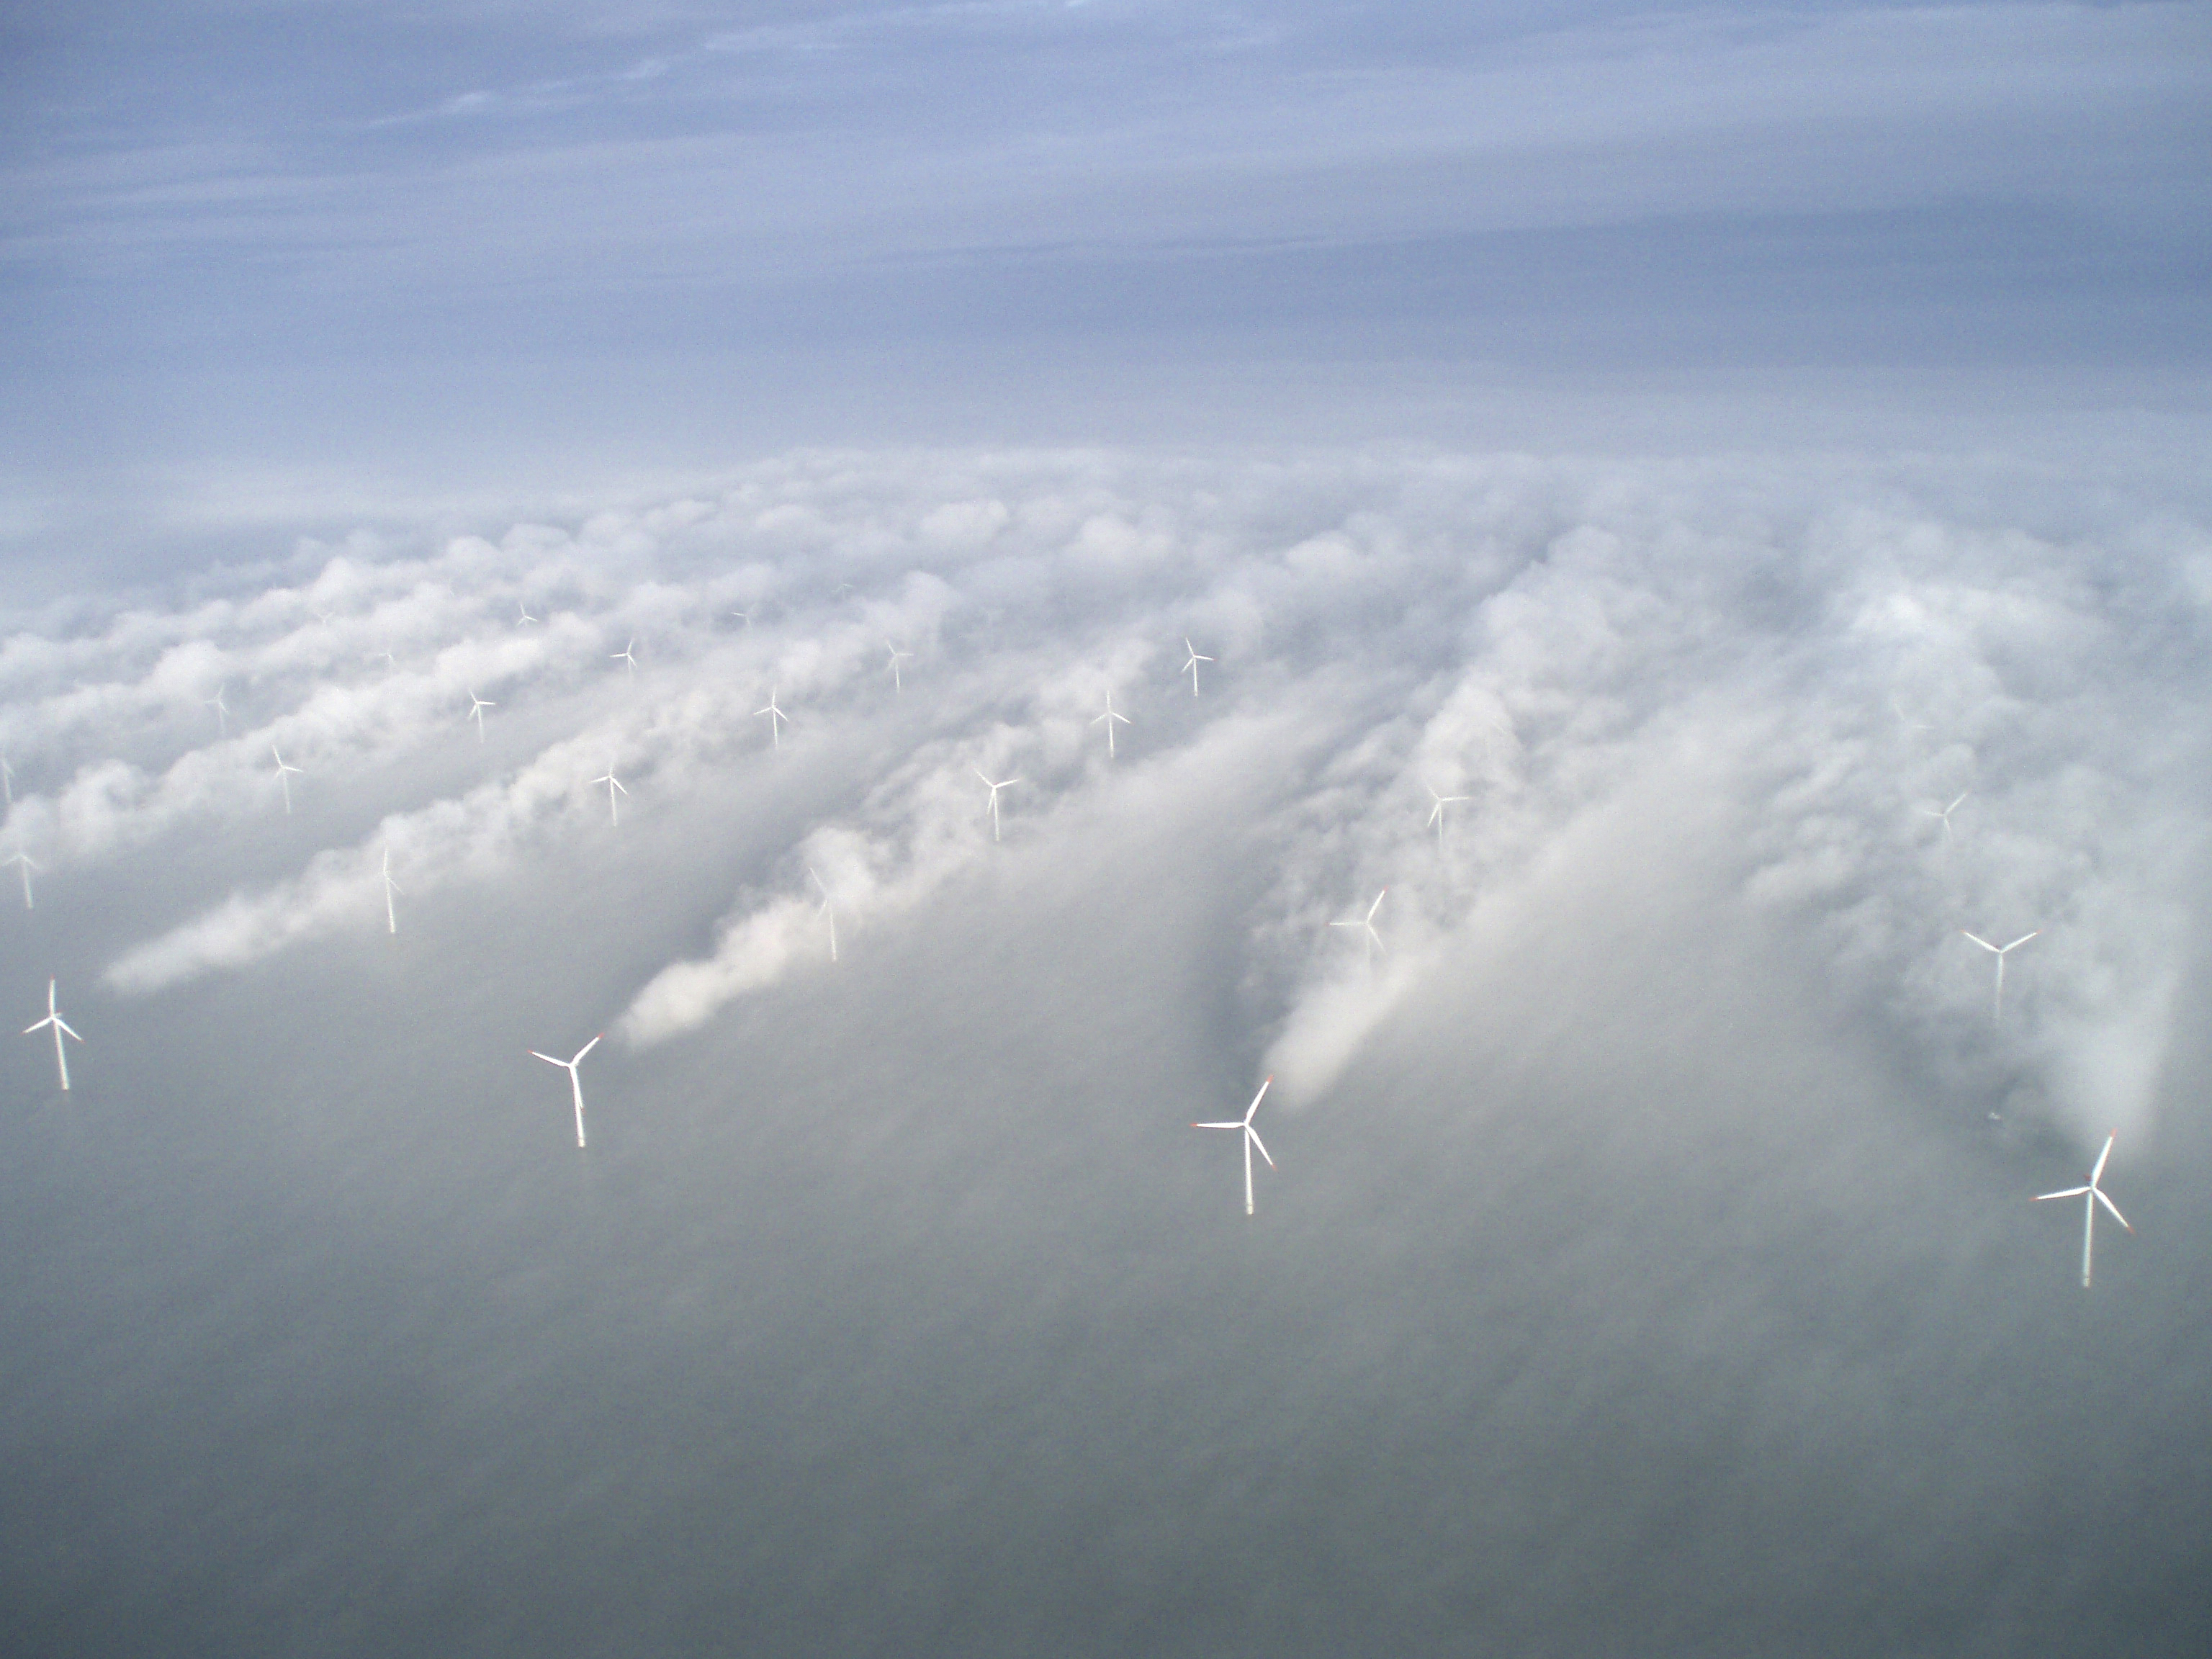
\includegraphics[width=\textwidth]{figs/intro/horn_revs_vattenfall.jpg}
    \label{fig:hornsrev-photo}
    % \caption{}
    \end{subfigure}
    \begin{subfigure}{0.5\textwidth}
        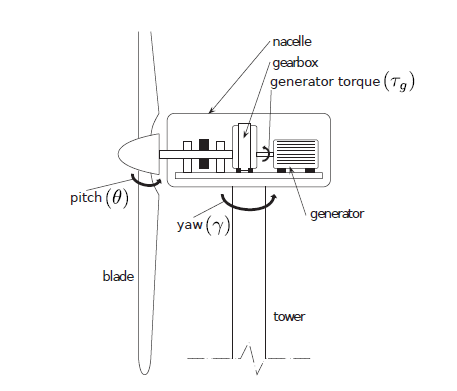
\includegraphics[width=\textwidth]{figs/intro/turbine_actuators.png}
    \label{fig:turbine_actuators}
    % \hfill
    \end{subfigure}
    \caption{Left: Wake effects in the offshore wind farm of Horns Rev 1 - Vattenfall. Right: Schema of a wind turbine \cite{boersma2017tutorial}. The \textit{pitch}, \textit{yaw} or \textit{torque} can be controlled.}
    \label{fig:intro-photos}
\end{figure}
% \md{Several actuators can be used to mitigate wake effects.
% Wind turbines can deflect their wakes away from downstream turbines by either tilting the rotor plane or increasing the \textit{yaw}, defined as the angle between the rotor and the wind direction. Wind turbines can also dampen the decrease of wind velocity in the wake by decreasing their wind energy capture: they can increase their \textit{pitch}, the angle between the turbine blades and the incoming wind, or directly control the torque of the rotor. These different strategies all lead to an increase in available wind velocity, and therefore production for the downstream turbines, at the cost of reducing the production of the actuating turbines. Similarly, misalignment with the wind direction for the yawed turbine leads to asymmetric increases of load for the upstream turbine \cite{cardaun2019analysis}, while the reduction of turbulence in the wake can alleviate fatigue on the downstream turbine. However, if a partial deflection of the wake is sufficient to increase the production at the downstream turbine, it can also add to its fatigue by increasing the variation in turbulence in front of its rotor \cite{stanley2022model}, while more frequent changes in actuation also increase the fatigue on actuators. These actuators can be used in the cooperative control of the wind farm to achieve different objectives, including the maximization of the total production, the minimization of loads to reduce maintenance costs over the wind turbine life-cycle \cite{wfc-quant-review}, or, as wind energy becomes a larger part of the energy mix, the tracking of power or frequency targets that will allow operators to offer ancillary services for grid integration \cite{miller2010advanced}. } 

% \md{Finding optimal control strategies is however hard. It requires computing wind statistics in front of every turbine rotor, which depend on complex aerodynamics governing the propagation of the wakes and their interactions in the field. No correct solution is known, and models tractable for classical optimization strategies must sacrifice fidelity, especially as the dimension of the problem explodes on large wind farms. Moreover, the optimal yaws found with respect to each model vary significantly with modeling choices. This has motivated developing model-free algorithms that can learn online in the real wind farm.}
%It requires describing the propagation of the turbulent wind flow across the farm to predict wind conditions in front of every turbine, and . An analytic expression is unknown, existing static models have large errors 
%and very hard to model at a cost reasonable computational cost for optimization, especially as the dimension of the problem explodes on large wind farms. 
%by bypassing the complex issue of modeling wind turbulences in the field to learn optimal control strategies online, RL algorithms can increase the efficiency of wind farms. 

The wind farm control problem is challenging. Conventional model-based control strategies require tractable models of complex dynamic interactions between turbines, and suffer from the curse of %dimension
dimensionality when the number of turbines increases. Moreover, optimal strategies differ significantly with modeling choices.
Reinforcement Learning (RL) provides a model-free, data-based alternative,
and recent work applying RL algorithms to wind farm control has yielded promising results (see e.g. \cite{abkar2023_rlwfc}). 
Single agent approaches, where a single RL controller must learn a centralized policy, encounter scaling challenges \cite{dong2023reinforcement}, are slow to converge under dynamic conditions \cite{liew2023_rl} and do not explore the graph structure of the problem induced by local perturbations. Several multi-agent RL approaches have been proposed to tackle this issue, relying on both centralized critics \cite{deng2023decentralized,dong2023reinforcement,padullaparthi2022falcon} and independent learning approaches \cite{dfac, kadoche-marlyc, stanfel_qlearning}. Authors have published code relative to their specific applications \cite{verstraeten2019fleet,verstraeten2021scalable,neustroev2022deep}, and \cite{neustroev2022deep} proposes a single-agent RL environment for power maximization in static simulations. There is to the best of our knowledge no open-source reinforcement learning environment for the general wind farm control problem.
%In part\cite{neustroev2022deep}, a single-agent RL environment for yaw-based power maximization is open-sourced, but only support 
%static simulation with global observation
%In particular \cite{neustroev2022deep} open sources a single-agent RL environment, but focuses on power maximization and only support static simulations.
%local observations. 
%focus on a single objective, do not propose realistic wind farm layouts or account for different optimization objectives, different simulation fidelity or decentralized control. There is to the best of our knowledge no open-source reinforcement learning environment for the general wind farm control problem.
%Different authors have published code relative to their specific applications, 
%In \cite{neustroev2022deep}, the authors have published their code for a specific problem, but they focus on a specific problem
% \jz{Why not cite as well your CDC paper ?}
%\md{These authors however formalize the reinforcement learning problem differently, evaluate their methods on different models, wind farm layouts or wind conditions.}
%
%Yet the lack of a common RL benchmark case prevents a fair assessment of the progress made so far: 

In this article, we propose WFCRL, the first open suite of reinforcement learning environments for the wind farm control problem. WFCRL is highly customizable, allowing researchers to design and run their own environments for both centralized and multi-agent RL. 

%In WFCRL, we frame a cooperative Multi-Agent Reinforcement Learning (MARL) problem: each turbine is an agent and can learn to adjust its yaw, pitch or torque to maximize the common objective.

% either tilt the rotor plane or 
Wind turbines can be controlled in several ways. A turbine can adjust its \textit{yaw} (defined as the angle between the rotor and the wind direction) to deflect its wake, increase its \textit{pitch} (the angle between the turbine blades and the incoming wind) to decrease its wind energy production, or directly control the \textit{torque} of its rotor. WFCRL makes it possible to control yaw, pitch or torque, and a schema of these different control variables can be found in \Cref{fig:intro-photos}. WFCRL offers a large set of observations including local wind statistics, power production, and fatigue loads for each turbine.
This makes it possible to consider different objective, including the maximization of the total production, the minimization of loads to reduce maintenance costs over the wind turbine life-cycle \cite{wfc-quant-review}, or, as wind energy becomes a larger part of the energy mix, the tracking of power or frequency targets that allows operators to offer ancillary services for grid integration \cite{miller2010advanced}. 

In WFCRL, interfaces with two state-of-the-art farm simulators are implemented : a static simulator FLORIS \cite{floris} and a dynamic simulator FAST.Farm \cite{fast.farm}. Indeed, the choice of a static or dynamic model is particularly important: the overwhelming majority of proposed approaches are evaluated on static models, but it was shown in \cite{stanfel_2021} that successful learning approaches under static conditions generally do not adapt to dynamic ones.
%\md{transfer to} \jz{have good performance on}  
%\jz{or optimal control strategies}
%\md{We should also expect significant differences between policy performances on static models as opposed to the real world, 
%and although realistic dynamic models are often too slow to allow online RL algorithms to learn from scratch,
%the transfer of pre-trained algorithms from the static to the dynamic case has not been studied. }
However, online learning from scratch with dynamic simulators is often too slow, making transfer learning from static to dynamic simulators of great interest.
From the broader literature on transfer learning and learning from simulators we know that it is challenging to train policies that can improve on previously learned behavior when deployed on new environments with unseen dynamics \cite{zhu2023transfer, hofer2021sim2real}. In spite of this problem, to the best of our knowledge, most approaches so far have been trained and evaluated on the same environment, and it is therefore not clear whether the policies learned with simulators are robust enough to be useful, or even safe, when deployed on real wind farms. With two simulators of different model-fidelity (referring to how closely the model represents the real system), WFCRL offers the possibility of designing transfer learning strategies between these simulators.

%parameterized with neural networks are prone to the catastrophic forgetting
%
%
%
%several works start to go towards MARL for wfc -  several challenges: dynamic conditions and load, => also a nice occasion to test exploitation of model knowledge - and yet, zero common benchmark !!
\subsection*{Contributions of the paper}
\begin{itemize}
    \item We introduce WFCRL, the \textbf{first open reinforcement learning} suite of environments for \textbf{wind farm control}. WFCRL is highly customizable, allowing researchers to design and run their own environments for both centralized and multi-agent RL. It includes a default suite of wind farm layouts to be used in benchmark cases.
    \item We interface all our wind farm layouts with \textbf{two different wind farm simulators}: a static simulator FLORIS \cite{floris} and a dynamic simulator FAST.Farm \cite{fast.farm}. They can be used to \textbf{design transfer learning strategies}, with the goal to \textbf{learn robust policies that can adapt to unseen dynamics}.
    \item We include implementations of three state-of-the-art MARL algorithms, IPPO, MAPPO \cite{yu2022surprising},  and QMIX \cite{rashid2020monotonic} adapted to our environments.
    \item We propose a benchmark example for \textbf{wind power maximization} with two wind condition scenarios. It takes into account the costs induced by wind turbine fatigue.
    % 
    %\item We propose a \textbf{wind power maximization benchmark} with two wind conditions scenarios and \textbf{evaluate two PPO-based state-of-the-art MARL algorithms}, IPPO and MAPPO.
    %
\end{itemize}

% \textcolor{blue}{TODO: introduce rest}

The paper is organized as follows. In \Cref{sec:wfcrl_suite}, we introduce the WFCRL environment suite. First in \Cref{subsec:environments} we introduce the simulators, the specifications of the simulated wind farms and turbines and the wind conditions scenarios we consider. We then lay out in \Cref{sec:marl} the cooperative MARL framework for the wind farm control problem, and finally detail the learning tasks and algorithms available with the suite in \Cref{sec:bench-learning}. In the second part \Cref{sec:benchmark}, we illustrate the possibilities of the WFCRL environment suite by introducing a benchmark example: the maximization of total power production with fatigue-induced costs. In \Cref{sec:bench-problem}, we explicit the actions, observations and rewards used in this problem, then in \Cref{subsec:bench-results}, we present and discuss the results of the IPPO and MAPPO on our benchmark tasks. In \Cref{section:discussion}, we discuss perspectives and limitations, and we conclude in \Cref{sec:conclusion}

%\section{Wind farm control as a Multi-Agent Reinforcement Learning Problem}
\section{WFCRL environments suite} \label{sec:wfcrl_suite}
% \md{In the following, we will consider the problem of power output maximization in wind farms. We emphasize however that we have designed our environments to be compatible with other objectives, in so far that the reward always depends on current productions and load measurements, our environments allow the reward function to be modified easily.  
%
% We consider a wind farm where $M$ wind turbines are operating in the same wind field and create turbulences that propagate across the farm. In a multi-agent approach, each turbine can be considered as an agent observing local properties of the wind field and the state of its own actuators, and all must cooperate to maximize the total wind production of the farm. This can be formulated as a Decentralized Partially Observable Markov Decision Process. In the following, we start a quick reminder of this Reinforcement Learning formulation, and then introduce the logic of our environment. }
In this section, we present our WFCRL environments suite.
We first present the simulators interfaced in WFCRL  (FLORIS and FAST.Farm), several pre-defined layouts and wind condition scenarios. 
Note again that having two simulation environments with different model-fidelity offers the possibility of designing transfer learning strategies between simulation environments.
Then, we describe briefly the MARL framework for the wind farm control problem. More precisely, we consider a wind farm with $M$ turbines, which operate in the same wind field and create turbulence that propagates across the farm. In our multi-agent environment, each turbine is considered an agent receiving local observations, and all cooperate to maximize a common objective. Note that WFCRL also has a single-agent RL environment, which uses global observations and actions.
%This can be formulated as a Decentralized Partially Observable Markov Decision Process.%Finally, we present our benchmark problem: the total power maximization problem.

\medskip

\subsection{The simulation environments}\label{subsec:environments}
In WFCRL, users can choose one of the two state-of-the-art wind farm simulators (FLORIS or FAST.Farm), select a pre-defined wind farm layout or define a custom one, and choose one of the implemented wind conditions. 
%\md{Every wind far simulation case - a set of wind conditions for a given layout - can be simulated with either one of two simulators: the steady-state FLORIS  \cite{floris} or the realistic dynamic FAST.Farm \cite{fast.farm}. }
%
% \textcolor{blue}{TODO: possible to add custom layout / simulator + contrôle 1 seul agent => done}
%A variety of simulators for wind farms have been developed. They 

Various wind farm simulators can be used to evaluate wind farm control strategies \cite{wake-models}. The choice of the wind farm simulators included in WFRCL relies on three criteria: the trade-off between fidelity and computation time, the popularity of the simulators in the wind farm energy community, and open-source availability. We discuss this further in \Cref{appendix:floris-fastfarm}, and introduce our simulation environments in the following paragraph.
%We chose to develop our environments on both FLORIS and FAST.Farm, two popular solutions of different levels of fidelity.
\paragraph{FLORIS environments}
%\md{Our first environment use the steady-state wind farm modeling introduced by the FLORIS. This set of models }
The wind farm simulator FLORIS implements static wind farm models, which
predict the locations of wake centers and velocities at each turbine 
%\md{and derive the production values as a function of the states of acuators at all rotors \cite{floris}. }
in the steady state: the dynamic propagation of wakes are neglected. The yaws of all wind turbines can be controlled, and the power production of the wind farm is then a function of all yaw angles and the so-called free-stream wind conditions: wind measurements - e.g. velocity and direction - taken at the entrance of the farm. FLORIS has been released as an open-source Python software tool\footnote{https://nrel.github.io/floris/}. In WFCRL environments built on FLORIS, global and local states contain time-averaged, steady-state wind and production statistics for both global and local observations. 

The models used by FLORIS do not compute any estimate of fatigues on wind turbines, and we propose to use local wind statistics to compute a proxy for load estimates indeed. We detail this when introducing our benchmark example in \Cref{sec:bench-problem}. 
%
%%\jz{A reference on the loads in FLORIS ?}
%\jz{Question: we can also control pitch and torque in FLORIS ?}
%
% \md{Our load penalty is therefore:
% \begin{equation}\label{eq:reward_load_floris}
%     r^L_{k, S} = \frac{1}{M} \sum_i^M \left(\sum_j^9 TI_{k}[x_{i,j},y_{i,j}] \right) + \frac{1}{M}  \sum_i^M \Bigg( \sigma(u_k[x_{i,j},y_{i,j}]) + \sigma({v_k[x_{i,j},y_{i,j}]}) + \sigma({w_k[x_{i,j},y_{i,j}]}) \Bigg)
% \end{equation}
%
% where $TI_k$ is the turbulence field at time-step $k$, $u_k$, $v_k$ and $w_k$ are respectively the $x$, $y$ and $z$ components of the velocity field as time-step $k$, and the $x_{i,j}$ define the coordinates of the $ 9 \times M$  grid points at which these values are computed for the $M$ rotor planes. } \jz{These penalties are to moved to the rewards in MARL problem..}
%
%
\paragraph{FAST.Farm environments}
Unlike FLORIS, FAST.Farm is a dynamic simulator that produces time-dependent wind fields that take into account the dynamics of wake propagation \cite{fast.farm}: wakes in wind farms tend to meander, and the wakes of different turbines interact and eventually merge as they propagate in the farms. One consequence is that under dynamic conditions there is a significant delay between the time agents take an action and the time this action finally impacts the turbines downstream.
%

FAST.Farm is built on wind turbine simulation tool OpenFAST \cite{openfast} which computes an estimate of the strength of the bending moment on each turbine blades. This reflects the structural loads induced on turbine blades, and thus can be used to design rewards in RL problems to reduce or avoid physical damages to turbines.
% \md{We directly use these estimates as a proxy for the structural loads induced on the turbines, and return the load penalty:
%
% \begin{equation}\label{eq:reward_load}
%     r^L_{k, D} = \frac{1}{M} \sum_i^M  \Bigg( \sum_j^3 |Mop_k[i,j]| + \sum_j^3 |Mip_{k}[i,j]| \Bigg)
% \end{equation}

% where $Mop_{k}$ is the $M \times 3$ matrix of out-of-plane bending moments for the $3$ blades of every turbine at time-step $k$, and $Mip_{k}$ is the corresponding matrix of in-plane bending moments.}
%
FAST.Farm is coded in Fortran. To allow for integration with the large ecosystem libraries and RL research practices developed in Python, we implement an interface between the simulator and the Python wind farm environment via MPI communication channels. The details of the interfacing infrastructure are reported in \Cref{appendix:interface}.

%md{In the following, we consider that all wind turbines are instances of the NREL Reference 5MW wind turbine} 
%\md{add} 
\paragraph{Wind farm layouts}  
Any custom layout - the arrangement of the wind turbines in the farm - can be used in WFCRL. We also propose several pre-defined wind farm layouts for use in benchmark cases. The coordinates of the wind turbines of $5$ real wind farms with $7$ to $91$ wind turbines are obtained from \cite{abritta2023plants}. A complete list of all correspondences between wind farms inspired by real environments and their locations is in \Cref{tab:wf-real}, and a list of all available environments can be found in \Cref{appendix:envs}. We also include in WFCRL several toy layouts, including a simple row of $3$ turbines  (the \textit{Turb3Row1} layout) for validation purpose and the $32$ turbines layout of the \textit{FarmConners} benchmark \cite{gocmen2022farmconners}. 
A visual representation of the %environment 
layouts can be found in \Cref{appendix:layouts}.
%An overview of some environments layout can be found in \Cref{fig:layouts}.

For all cases, we simulate instances of the NREL Reference 5MW wind turbines, whose specifications have been made public by the National Renewable Energy Laboratory (NREL) \cite{jonkman2009definition}. It has become standard reference for wind energy research and is used by the majority of proposed evaluations of RL methods \cite{abkar2023_rlwfc}. 
%\jz{Question: other turbines can be defined ?}

% \begin{figure}
%      \centering
%      \begin{subfigure}{0.3\columnwidth}
%      \includesvg[width=\columnwidth]{figs/layouts/layout3TurbRow1.svg}
%      \caption{Toy case: Row of $3$ turbines}
%      \end{subfigure}
%      \begin{subfigure}{0.3\columnwidth}
%      \includesvg[width=\columnwidth]{figs/layouts/layoutAblaincourt.svg}
%      \caption{Ablaincourt}
%      \end{subfigure}
%      \begin{subfigure}{0.3\columnwidth}
%      \includesvg[width=\columnwidth]{figs/layouts/layoutOrmonde.svg}
%      \caption{Ormonde}
%      \end{subfigure}
%      \begin{subfigure}{0.3\columnwidth}
%      \includesvg[width=\columnwidth]{figs/layouts/layoutWMR.svg}
%      \caption{WMR}
%      \end{subfigure}
%       \begin{subfigure}{0.3\columnwidth}
%      \includesvg[width=\columnwidth]{figs/layouts/layoutHornsRev1.svg}
%      \caption{Horns Rev 1}
%      \end{subfigure}
%      \begin{subfigure}{0.3\columnwidth}
%      \includesvg[width=\columnwidth]{figs/layouts/layoutHornsRev2.svg}
%      \caption{Horns Rev 2}
%      \end{subfigure}
% \caption{Coordinates of each wind turbine for the layouts of some wind farm environments implemented in WFCRL. Distances are in $km$ and the distance between two adjacent grid lines (resp. columns) is of $1$ turbine diameter.}
%  \label{fig:layouts}
% \end{figure}
%
\begin{table}
    \centering
    \begin{tabular}{c|c}
         \textbf{WFCRL environment} & \textbf{Real wind farm} \\
         Ablaincourt &  Ablaincourt Energies onshore wind farm, Somme, France \\
         Ormonde & Ormonde Offshore Wind Farm, Irish Sea, UK\\
         WMR & Westermost Rough Wind Farm is an offshore wind farm, North Sea, UK \\
         HornsRev1 & Horns Rev 1 Offshore Wind Farm, North Sea, Denmark\\
         HornsRev2 & Horns Rev 2 Offshore Wind Farm, North Sea, Denmark\\
         &\\
    \end{tabular}
    \caption{Correspondences between WFCRL environments and real wind farms.}
    \label{tab:wf-real}
    \vspace{-2em}
\end{table}
%
%, and the length on an episode corresponds to the time under a set of wind conditions
\paragraph{Wind condition scenarios}
For all environments, we distinguish three scenarios. 

\textit{Wind scenario I:}
In this scenario, all trajectories in a given environment are run under the prevailing wind velocity and direction at the location. 

\textit{Wind scenario II:}
In this scenario, we let the wind farm be subject to variations in wind change, and sample new free-stream wind conditions $u_\infty, \phi_\infty$ at the beginning of each episode: 
\begin{equation}
%\begin{split}
    u_\infty \sim \mathcal{W}(\bar{u}, \lambda) \quad
    \phi_\infty \sim \mathcal{N}(\bar{\phi}, \sigma_\phi)
%\end{split} 
\end{equation}
where $\mathcal{W}$ is a Weibull distribution modeling wind speed with shape $\lambda$ and scale $\bar{u}$, and $\mathcal{N}$ is a Normal distribution with $\bar{\phi}$ being the dominant wind direction for a given farm. 

\textit{Wind scenario III:}
In this scenario, the wind farm is subjected to a an incoming wind that varies during a single episode. Any time series with wind speed and direction measurements can be used by WFCRL, and we provide a default time series of measurements collected on a real wind farm. A starting point in the time-series is randomly selected at the beginning of each new episode.

%\md{At the start of each episode, all wind turbines are aligned with the wind direction.}
By default, at the beginning of each simulation, all wind turbines have the yaw angle zero.
This corresponds to the so-called \textit{greedy} case, the strategy that would allow each of them to maximize its production in un-waked conditions.

%We then distinguish the environments by the simulation by the simulator used to model wake interactions and compute the wind field. 
%
%We now introduce the MARL framework used to design our environments.
%
%
%\subsection{Preliminaries }
\subsection{The MARL framework for the wind farm control problem}\label{sec:marl}

A Decentralized Partially Observable Markov Decision Process (Dec-POMDP) with $M$ interacting agents is a tuple $\{M, S, O, A, P, o^1, \dots, o^M, r\}$. $S$ is the full state space of the system, while for any $i \in \{ 1, \dots, M \}$, $O_i$ is the observation space of the $i$th agent with $O = \times_{i}^M O_i$. $A_i$ is the local action space of the agent, and the global action space is the product of all local action spaces $A = \times_{i}^M A_i$.  
At each iteration, all agents observe their local information, chose an action and receive a reward $r : S \times A \times S \rightarrow \mathbb{R}$. The system then moves to a new state, which is sampled from the transition kernel $P : S \times A \times S \rightarrow [0,1]$. $P$ gives the probability of transition from a state $s \in S$ to $s' \in S$ when agents have taken global action $a \in A$. The probability for the $i$th agent to observe $o_i$ is then defined by local observation function $o^i: S \times A \times O_i \rightarrow [0,1]$, and the history of all past observations is denoted $h_i$.
%all agents have collectively taken global action $a \in A$.
We call $\pi_1, \dots, \pi_M$ the policies followed by each agent, where $\pi_i(a_i | h_i)$, defines the probability for agent $i$ to chose action $a_i$ after observing $h_i$. The corresponding global policy $\pi = (\pi_1, \dots, \pi_M)$ simply concatenates the outputs of all local policies. 
% \jz{Note that agents have the same objective, but their rewards can be different from each other. Mais ce n'est plus un Dec-POMDP ? }
%
\paragraph{Objective} The MARL problem is to
%The goal is to 
find a policy $\pi^*$ that maximizes the expectation of the discounted sum of rewards collected over a finite or infinite sequence of time-steps
\begin{equation} \label{expected_cost}
    \max_{\pi} \mathbb{E}_{s_0, a_0, s_1, \dots} \left[ J \right], \quad J:= \sum_{k=0}^T \beta^k r_k
\end{equation}
with  $0 < \beta < 1$ the discount factor and $T$ the number of steps in the environment, or the length of an episode.
For the wind farm control problem, possible rewards include the total production of the farm or a distance to a target production. As fatigue load measurements are also available, rewards can be designed to encourage actions that preserve the turbine structure. Note that knowledge of the farm layout and incoming wind direction can also be exploited to represent wake interactions between wind turbines as a time-varying graph (see \Cref{appendix:graph}): this approach can motivate the design of local reward functions for decentralized learning RL algorithms with communication. Moreover, empirical successes applying RL to wind farm control have often relied on creative reward shaping \cite{abkar2023_rlwfc,drl-high-fidelity}. To support these two efforts, WFCRL implements a \texttt{RewardShaper} class that allows easy design of custom reward functions, and can be used to train both centralized and decentralized learning algorithms.

%\subsection{The MARL framework}
%We now formalize the wind farm control problem within this framework, and introduce the logics of our environment.
%\md{3D}  \md{obviously} 
%\md{which is a partial observation of the full state}
\paragraph{State and Observation} 
%\textcolor{blue}{TODO: Add local/global state schema ?}
As the production of each turbine is a function of the local wind conditions at its rotor, a Markovian description of the full state of the system should contain the whole wind velocity field of the entire farm. This is impossible to know in practice.
%\md{ Rather, each turbine has an anemometer that measures the wind speed and direction at its rotor, and a partial observation of the global state can be reconstituted by combining all local observations. }
We rather assume that local measurements of wind speed and direction are available at each wind turbine, and that an estimate of the free-stream wind speed and direction can be accessed, but might not necessarily be sent to the turbines in real time. 
Our environments therefore distinguish between the local observations $o_i$ for each i $ \in \{1, \dots, M\}$ and a global observation $o_g$. 
Each $o_i = (u_i, \phi_i, \theta_i)$ contains a local measure of the wind velocity $u_i$ and direction $\phi_i$, as well as the last target value sent to each actuator $\theta_i$. On FLORIS environments, $\theta_i$ is always equal to the current value of the actuators. This is not the case on FAST.Farm, for which an inner control loop at the level of the actuators adds a response delay. The global observation $o_g = (o_i, \dots, o_M, u_\infty, \phi_\infty)$ contains the concatenation of all local states, as well as the free-stream measure of the wind $u_{\infty}, \phi_{\infty}$. \Cref{tab:summary_obs_actions} summarizes all observations and actions available with the two simulators.
%\jz{Question: The design of observations, for me, should be a part of the RL designers' work. The description here seem to limite the imagination of researchers. For example, DFAC has a different local observation.}
%
% In a Centralized Training and Decentralized Execution (CTDE) framework, the global observation could for example be accessed at training time, an example of th
% \textcolor{blue}{TODO: link with MAPPO ?, more on simulator as proxy vs simulator as training ground}
%
%
\begin{table}
    \centering
    \begin{tabular}{c|c|c}
        & FLORIS & FAST.Farm  
        \\ \hline %\bottomrule\\
         Local Observations $o_i $&  $u_i, \phi_i$ (steady-state), $y_i$ & $u_i, \phi_i$ (time-dependent), $y_i, p_i, \tau_i$ \\
         Global Observations $o_g$ & \multicolumn{2}{c}{$o_1, \dots, o_M, u_{\infty}, \phi_{\infty}$}\\
         Actions & 
         $\Delta y_i$ & $\Delta y_i, \Delta p_i, \Delta \tau_i$ \\
         \hline
    \end{tabular}
    \caption{Observations (global and local) and actions available for an agent $i$ in FLORIS and FAST.Farm environments. $y_i, p_i, \tau_i$ refer respectively to the yaw, pitch and torque of the turbine.}
    \label{tab:summary_obs_actions}
    \vspace{-2em}
\end{table}
%\jz{Question: As we have introduced the simulators, now we can list all possible elements for the observations for the two environments. In a Table ?}
%
% \md{Wind turbines can use several actuators to mitigate the impact of their wakes. 
%Three different ones are considered here}
\paragraph{Actions}
WFCRL offers several ways to control wind turbines: the \textit{yaw}, the \textit{pitch} or \textit{torque}. Yaw control is available on the FLORIS environments, and all three can be controlled on FAST.Farm environments. The yaw is the angle between a wind turbine's rotor and the wind direction: turbines facing the wind have a yaw of $0\degree$ which maximizes their individual power output. Increasing the yaw can deflect the wake away from downstream turbines, which may increase the total production of the wind farm. 
The pitch is the angle of the attack of the rotor blades with respect to the incoming wind, while the torque of the turbine's rotor directly controls the rotation speed. Increasing the blade pitch or decreasing the torque target both decrease the fraction of the power in the wind extracted by the turbine, and therefore decrease the turbulence in its wake. 
To reflect the fact that the actuation rate of the wind turbines is limited by physical constraints, we conceive actions as increases or decreases in the actuator target value rather than absolute values, with the limits being implemented by the upper and lower bounds of a continuous action space. 
%\jz{Question: other action definition is possible ? If so, better to say that we define by defaut ... but other definitions are also easy to implement.} 
%\jz{Question2: does FLORIS has also these three control options ?}

\subsection{Learning in WFCRL}\label{sec:bench-learning}

%\paragraph{Implementation} 
All environments are implemented with standard RL and MARL Python interfaces Gymnasium \cite{openai-gym} and PettingZoo \cite{pettingzoo}. The source code of WFCRL is open-sourced under the Apache-2.0 license and publicly released at \url{www.github.com/ifpen/wfcrl-env}. 
%The code to reproduce all experiments is available at \url{www.github.com/ifpen/wfcrl-benchmark}.

\subsubsection{Online Learning}\label{sec:bench-online}

Environments implemented on both FLORIS and FAST.Farm can be used in an episodic learning approach. This is the traditional setting of the RL problem, and we will refer to it as the \textit{Online Learning} Task.
%\md{In the first scenario}
% where agents learn to cooperate against a single set of wind conditions,
In Wind scenario I and III, we look at the evolution of the sum of rewards collected over an episode. 
%\md{In the second scenario} 
In Wind scenario II, where a different set of wind conditions is sampled at each episode, we evaluate the policies on a predefined set of wind conditions and use a weighted average as the final score. This gives us our evaluation score:
%
\begin{equation}\label{eq:eval_eq}
    \texttt{score}(\pi_1, \dots, \pi_M) = \sum_{j=1}^{n_w} \rho_j  \sum_{k=0}^T r_k
\end{equation}
%
where $T$ is the length of the episode,  $n_w$ is the number of wind conditions considered and the $\rho_1, \dots, \rho_{n_w}$ are the weights on each conditions, with for all $j$, $ 0 < \rho_j < 1$ and $\sum_j^{n_w} \rho_j = 1$. The wind conditions distributions on which policies are evaluated need not be identical to the one from which conditions were sampled during training.

\subsubsection{Transfer}\label{sec:bench-transfer}
%\md{can be considered} 
Exploration on real wind farms is costly: as prototype models are typically not available for large wind farms, adjusting to the real dynamics of the system will require exploring in real time on an operating wind farm. Every move of explorating in a suboptimal direction is a cost for the farm operator. Learning efficient policies offline that can quickly adapt to the real system is therefore critical. Since the dynamic FAST.Farm simulator is considered a higher fidelity version of the static simulator FLORIS, we propose to use the former as a proxy of a real wind farm to evaluate the robustness of policies learned on the latter, and their ability to adjust to the real dynamics of a farm. We will refer to this as the \textit{Transfer} Task.
%
%and the question of learning sufficiently robust policies offline that safely improve once deployed online in the field is still open
%
% \section{Benchmark Tasks}

\subsubsection{Algorithms}\label{sec:bench-algos}

We focus on two 
state-of-the-art
algorithms IPPO (Independent PPO) and MAPPO (Multi-Agent PPO) introduced in \cite{de2020independent, yu2022surprising}. Both are based on the on-policy actor-critic PPO algorithm \cite{schulman2017proximal}, and support continuous action spaces. Following an approach called independent learning, IPPO builds on PPO by allowing every agent to run a PPO algorithm in parallel. MAPPO, on the other hand, maintains both $M$ agent policies taking actions based on local information and a shared critic, which estimates the value of a global observation.  The choice of the global observation fed to the critic is an important factor influencing the performance of the algorithm \cite{yu2022surprising}. We follow the recommendations of \cite{yu2022surprising} to adapt PPO to the multi-agent case. They suggest to include both local and global observation features to the value function input. We therefore feed to our shared critic network the full global observation introduced in \Cref{sec:marl}, that is both the of concatenation of all local observations and the free-stream wind velocity.

In \cite{yu2022surprising}, it was found that PPO-based methods perform very well when extended to cooperative multi-agent tasks, outperforming algorithms specifically designed for cooperative problems like QMIX \cite{rashid2020monotonic}. We implement both QMIX and independent Deep Q-network (DQN) \cite{mnih2015human} baselines, where all agents run DQN algorithms in parallel using a discrete action space. As QMIX uses a recurrent neural network, we implement independent DQN baselines with both fully connected (IDQN) and recurrent (IDRQN) neural networks. The same global observation is fed to the central MAPPO critic and the mixing network of QMIX.
%\md{at the entrance of the farm}. 

For implementation, we adapt the CleanRL \footnote{https://github.com/vwxyzjn/cleanrl} \cite{huang2022cleanrl} baseline implementations of PPO and DQN to our multi-agent Petting Zoo environments. Although our analysis for the benchmark case considered in \Cref{sec:benchmark} focuses on PPO-based algorithms on continuous action spaces, additional results for baselines on discrete action spaces are  reported in \Cref{appendix:results}.
%implementations of two other baselines, Independent Q-Learning (IQL) and QMIX \cite{rashid2020monotonic}, are also available.
%although they are not 
%Since given a local observation the optimal policies are not identical for all turbines, we do not implement weight sharing between different agents. 

% \md{\textbf{Measures and Rewards}} } 
\medskip

%In order to illustrate the possibilities offered by our environments suite, we introduce a benchmark example in the next section.

\section{Benchmark example: the maximization of the total power production}\label{sec:benchmark}

%We implement a benchmark example in WFCRL. Recall that local observations, actions choice, and rewards can be customized easily in WFCRL.
%
We consider the problem of finding the optimal yaws to maximize the total power production under a set of wind conditions, and taking into account the costs induced by turbine fatigue load. This problem is known as the \textit{wake steering} problem, and is an active area of research in the wind energy literature \cite{houck2022review,howland2019windfarm}.

\subsection{Problem formulation}\label{sec:bench-problem}
%
%\md{Since we consider here the role of the maximization of the total power production of the farm in a cooperative context, we start by defining the shared reward as the total production of the farm.}
%
\paragraph{Actions and observations} Local observations include the local yaw and local wind statistics. The concatenation of all local observations along with free-stream wind statistics in the global observation is as described in \Cref{sec:marl}.
Recall that actions are defined as increase or decrease in the actuator target value. In this problem, all agents control their yaws, and we define the continuous action space $[-5,5]$, defining changes in yaw angle expressed in degrees. To constraint the load on the turbines caused by the control strategies and reduce its impact on the lifetime of the turbines, the time each turbine spends actuating is limited. We choose the upper bound of $10\%$ of the time, which is the same upper bound value discussed in \cite{puech2022improved}. At every iteration, the time needed to change the state of the actuator is computed, and any action violating this condition is not allowed.
%alignment with the wind direction for the yawed turbine leads to asymmetric increases of load for the upstream turbine \cite{cardaun2019analysis},

\paragraph{Rewards}
 At each iteration $k$, all agents receive a reward $r^P_k$ which is the currently measured production of the wind farm in kW divided by the number of agents and normalized by the free-stream wind velocity: 
%
\begin{equation}\label{eq:reward_production}
r^P_k = \frac{1}{M} \sum_i^M  \frac{\hat{P}^i_k}{(u_{\infty,k})^3} 
\end{equation}
where $\hat{P}^i_k$ is the measured power production and $u_{\infty,k}$ the free-stream wind velocity at time-step $k$.
%Under static conditions, this power production per definition corresponds to time-averaged predictions. Under dynamic conditions, we return $10$min time-averaged production values.
%\md{on this reward will be}
To discourage agents from taking risky policies damaging the turbines, we also return a load penalty $r^L_k$ which increases with the sum of loads on all the turbine blades. 
%Since the availability of load measurements depend on the chosen simulator, more details on this \jz{are} discussed in \Cref{subsec:environments}.
%if a partial deflection of the wake is sufficient to increase the production at the downstream turbine,
%while more frequent changes in actuation also increase the fatigue on actuators.

FLORIS does not provide estimates of the loads on structures. Instead, we evaluate the impact of actuations on loads with a proxy based on local estimates of turbulence and velocities on the surface of the rotor planes. Our proxy takes into account 2 factors increasing stress on wind turbine structures as noted in \cite{stanley2022model}: first, the turbulence of the wind and second, the variation of velocities on the turbine rotor. 
We therefore define the load penalty in FLORIS environments as 
\begin{equation}\label{eq:reward_load_floris}
    r^L_{k, S} = \frac{1}{M} \sum_i^M \left( \sum_j^9 TI_{k}[x_{i,j},y_{i,j}] + \sigma(u_k) + \sigma({v_k}) + \sigma({w_k})  \right)
    % r^L_{k, S} = \frac{1}{M} \sum_i^M \left(\sum_j^9 TI_{k}[x_{i,j},y_{i,j}] \right) + \frac{1}{M}  \sum_i^M \Bigg( \sigma(u_k[x_{i,j},y_{i,j}]) + \sigma({v_k[x_{i,j},y_{i,j}]}) + \sigma({w_k[x_{i,j},y_{i,j}]}) \Bigg)
\end{equation}
where $TI_k$ is the turbulence field at time-step $k$, $u_k$, $v_k$ and $w_k$ are respectively the $x$, $y$ and $z$ components of the velocity field at time-step $k$, and the $x_{i,j}$ define the coordinates of the $ 9 \times M$ grid points at which these values are computed for the $M$ rotor planes. $\sigma$ denotes the standard-deviation.
%The first component uses a steady-state estimation of turbulence on a grid of $9$ points taken on the plane of each turbine. 
%The second component reflects the fact that loads on turbine blades are impacted by partial waking, where after an upstream has increased its yaw, only a part of the rotor plane is still in its wake. 
%
\begin{figure} 
     \centering
     \begin{subfigure}[b]{0.45\columnwidth}
     \centering
     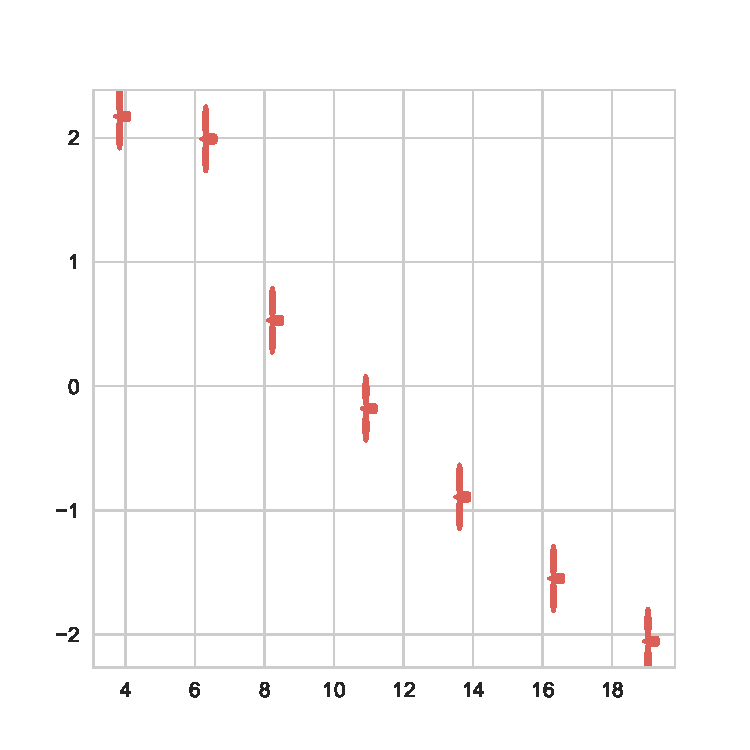
\includegraphics[width=\columnwidth, height=4cm]{figs/layouts/layoutAblaincourt.pdf}
     \vspace{0.5em}
     \caption{Ablaincourt Layout}
     \end{subfigure}
      \begin{subfigure}[b]{0.45\columnwidth}
     
\includegraphics[width=\columnwidth]{figs/wfixed/reward/Ablaincourt_Floris_constant_score.eps}
     \caption{Episode Reward}
     \label{fig:abl-layout}
     \end{subfigure}
     \begin{subfigure}[b]{0.45\columnwidth}
     
\includegraphics[width=\columnwidth]{figs/wfixed/powers/Ablaincourt_Floris_constant_score.eps}
     \caption{Power (MWH)}
     \end{subfigure}
     \begin{subfigure}[b]{0.45\columnwidth}
     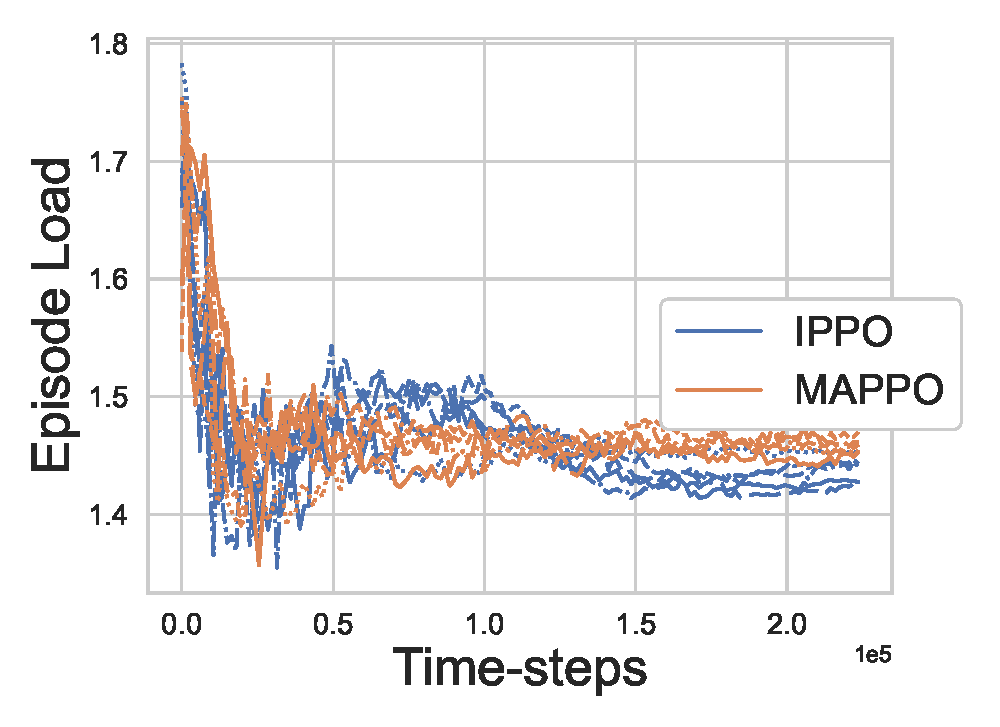
\includegraphics[width=\columnwidth]
     {figs/wfixed/loads/Ablaincourt_Floris_constant_score.eps}
     \caption{Load Indicator}
     \end{subfigure}
\caption{The evolution of total reward (b), power output (c) and load penalties (d) accumulated over an episode (with $T$=150) on the \textit{Ablaincourt} environment, simulated with FLORIS. A visual representation of the layout is in (a), where the coordinates are in wind turbine diameters. During training, policies are evaluated every $5$ training steps with deterministic policies. The curves are plotted for all $5$ seeds.}
 \label{fig:results}
\end{figure}

For FAST.Farm, we use the estimates of the the blades' bending moment strength as a proxy for the structural loads induced on the turbines, and define the load penalty as
\begin{equation}\label{eq:reward_load}
    r^L_{k, D} = \frac{1}{M} \sum_i^M  \Bigg( \sum_j^3 |Mop_k[i,j]| + \sum_j^3 |Mip_{k}[i,j]| \Bigg)
\end{equation}
where $Mop_{k}$ is the $M \times 3$ matrix of out-of-plane bending moments for the $3$ blades of every turbine at time-step $k$, and $Mip_{k}$ is the corresponding matrix of in-plane bending moments.

Both rewards are common to all turbines, and all must therefore maximize \eqref{expected_cost} with $r_k = (r^P_k - \alpha r^L_k)$, where $\alpha$ is a weighting parameter. The load penalty indicator returned by the environment is downscaled so that $r^P_k$ and $r^L_k$ are of similar magnitudes. By default, the value of $\alpha$ is $1$, but greater or less importance can be given to turbine safety by changing $\alpha$. 
%the current production energy and load-induced maintenance cost for wind energy projects.
%$\sum_{k=0}^T \beta^k (r^P_k - 0.1 r^L_k)$ with $T$ the number of steps in the episode, 
%corresponding to the value for which $r^P_k$ and $\alpha r^L_k$ are of the same magnitude.
%We moreover add a reward $r^I_k$ which returns the increase in percentage of the total production between two timesteps, finding that it greatly helps learning (add plot in Appendice) ? The agents should collectively maximize  

\paragraph{Wind conditions}
We focus here on Wind Scenarios I and II. To evaluate the algorithms on Scenario II with score \eqref{eq:eval_eq}, we need to define weights $\rho_j$. We use data acquired during the SmartEole project at the location of the Ablaincourt wind farm \cite{7turb-layout}. It consists of estimates of free-stream wind direction and velocity computed from measures taken during a $3$ months field campaign every $10$ min. Since in real conditions wind velocity and wind direction are correlated, we compute the bi-dimensional histogram for the two variables, taking $5$ bins for each dimension. We obtain a set of $25$ wind condition rectangles. The wind conditions $w_1, \dots, w_j$ are the center of each rectangle, and the corresponding weights $\rho_j$ are defined as the frequencies at which wind conditions in the time series appeared in the rectangle.
%
\subsection{Results}\label{subsec:bench-results}
%\md{We compare both their learning curves on FLORIS and evaluate their performance and transfer abilities on FAST.Farm. }
%
%
\begin{figure}
     \centering
     \begin{subfigure}{0.45\columnwidth}
     
\includegraphics[width=\columnwidth, height=4.5cm]{figs/xps_turb3/windrose/score_trainw.eps}
     \caption{\textit{Turb3Row1}}
     \end{subfigure}
     \begin{subfigure}{0.45\columnwidth}
     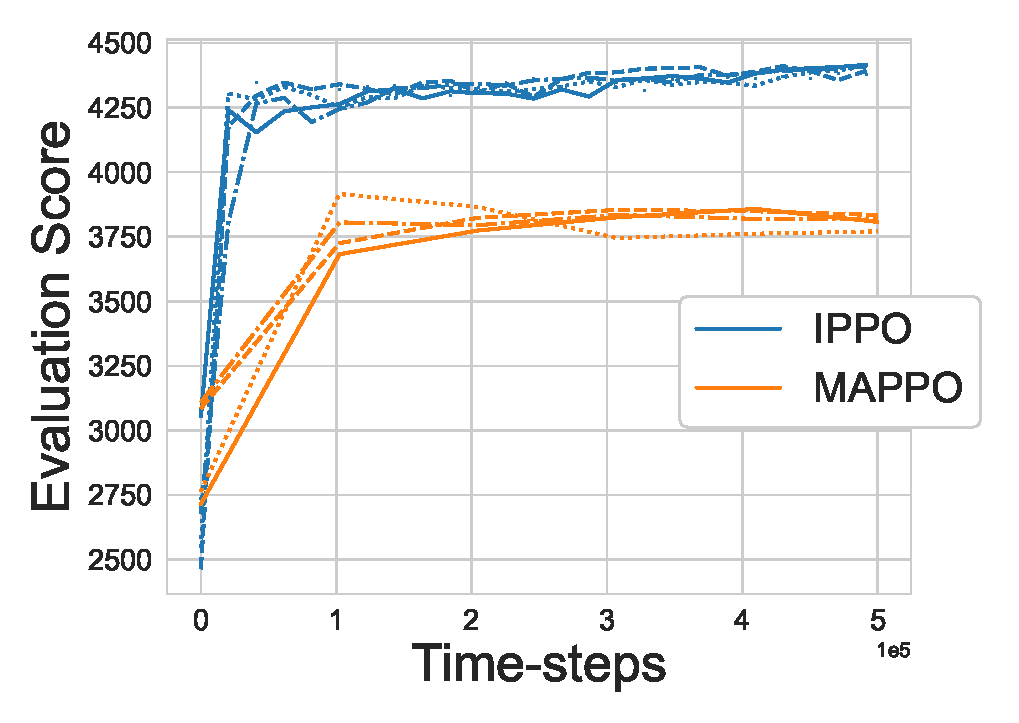
\includegraphics[width=\columnwidth, height=4.5cm]{figs/xps_ablaincourt/windrose/score_trainw.eps}
     \caption{\textit{Ablaincourt}}
     \end{subfigure}
\caption{Evolution of the evaluation score, defined in \eqref{eq:eval_eq}, during the training of IPPO and MAPPO on the two environments \textit{Turb3Row1} (left)  and \textit{Ablaincourt} (right).}
 \label{fig:eval_scores}
\end{figure}
%
%\md{The results on this preliminary benchmark are reported  in \Cref{tab:train_scores}. }
%%\Cref{tab:train_scores}.
%We distinguish two scenarios, the first (resp. second) is trained with the wind scenario I (resp. II) 
We apply algorithms IPPO and MAPPO, whose implementations are both available in WFCRL, to our benchmark example. Both are trained on the two wind scenarios I and II described in \Cref{subsec:environments}, on the static simulator FLORIS. For the Scenario I, the score is the reward obtained on a single policy rollout of $150$ steps in the environment, and policies are updated after $2048$ steps in the environment. Learned deterministic policies are evaluated every $5$ training steps. Results for the \textit{Ablaincourt} layout are given in Fig. \ref{fig:results}.
%We also report the change in percentage point of the average power output and load over the greedy baseline. 
For the Scenario II, the score is the one defined in \eqref{eq:eval_eq}, with $T=2048$.
The training curves for the the \textit{Ablaincourt} and the \textit{Turb3Row1} layouts are illustrated in Fig. \ref{fig:eval_scores}.

At the end of training, we evaluate all algorithms on both scenarios, as well as on FAST.Farm environments for Scenario I. On \textit{Turb3Row1}, IPPO has the best performance for all evaluation tasks, while on \textit{Ablaincourt}, MAPPO performs better for $2$ evaluation tasks out of $3$. This confirms the good empirical results of IPPO on cooperative tasks observed in the literature \cite{de2020independent}, and suggests that MAPPO's shared critic becomes more beneficial as the number of agents increases. Although IPPO and MAPPO perform similarly on Scenario I, the gap in favor of IPPO increases on Scenario II, showing MAPPO to be less efficient at adapting policies to diverse wind conditions.

%This is not always true when executing them on FAST.Farm.
As expected, the best evaluation performance for each wind scenario on FLORIS is provided by the algorithms trained on this scenario. Yet on FAST.Farm, although our evaluation task is solely under Scenario I (constant wind), its noisier wind observations pose a challenge to IPPO policies trained on Scenario I. As local wind observations are now perturbed by time-dependent turbulences created by other agents, information sharing (MAPPO) or exposition to a variety of wind conditions (Scenario II) during training becomes more useful. 
%On the other hand, IPPO performs significantly better than MAPPO on Scenario II evaluation task. 
%
%noisier observations and wind field turbulences induced by the agents 
%Although algorithms trained on Scenario II predictably perform better on 

A table detailing all evaluation scores at convergence is available in \Cref{appendix:results} and hyper-parameters are given in \Cref{appendix:training-details}. The code to reproduce all experiments is available at \url{www.github.com/ifpen/wfcrl-benchmark}.

To illustrate the \textit{Transfer} case, we then fine-tune the learned IPPO policies on a \textit{Turb3Row1} on $40k$ steps ($1$ day in simulated time) in the corresponding FAST.Farm environment. We report in \Cref{appendix:transfer-curves} the evolution of average power output and load, and compare it to a naive deployment of strategies learned online. Our results illustrate the difficulty of adapting learned policies to unseen dynamics.
%and we discuss them in t. 
 
%To illustrate the \textit{Transfer} case, we then deploy the learned IPPO policies on a \textit{Turb3Row1} on $40k$ steps ($1$ day in simulated time) in the corresponding FAST.Farm environment. We report in \Cref{appendix:transfer-curves} the average the evolution of power output and load, and compare it to a naive deployment of strategies learned online. Our results illustrate the difficulty of adapting learned policies to unseen dynamics.
%
% \begin{table}[]
%     \centering
%     \begin{tabular}{c|cc}
%     & \textbf{IPPO} & \textbf{MAPPO}\\
%     \bottomrule \\
%        \textit{Turb3Row1 (Sc. 1)}  & $1238	\pm 24$
%         & $1369 \pm 41$  \\
%         \textit{Turb3Row1 (Sc. 2)} & $1607 \pm	41$ &	$1369	\pm 124$ \\
%     \end{tabular}
%     \caption{FAST.Farm evaluation task}
%     \label{tab:fastfarm_transfer}
%     \vspace{-1.5em}
% \end{table}
% 
\section{Limitations}\label{section:discussion}
%\textbf{Simulators} 
As noted in \Cref{sec:wfcrl_suite}, the choice of the simulators included in WFRCL has been made on the criteria of fidelity, computation cost, popularity and availability in open source. Both FLORIS and FAST.Farm are developed and actively maintained by the US-based National Renewable Energy Laboratory \footnote{https://www.nrel.gov/}, and have a large user base among wind energy researchers. FAST.Farm was explicitly designed to provide good fidelity at a limited computation cost \cite{fast.farm}. Despite this, dynamic wind farm simulators remain slow. The development and open-sourcing of faster dynamic simulators will be critical. Machine-learning accelerated simulators could be an important step in that direction.
Moreover, although FAST.Farm has been extensively validated against both real wind farm data and high-fidelity simulations (see \Cref{appendix:floris-fastfarm}), there has been to the best of our knowledge no explicit investigation of the transfer of yaw optimization results from FAST.Farm simulations to a real wind farm.
%and serve as a intermediary between FLORIS and FAST.Farm. 
%> WFCRL simulators, most used and open source
%But dynamic simulators with good fidelity use by wind energy community are slow, => work done developing faster and new open-source simulators will be critical, could serve as a 3rd intermderiary simulator, other areas include developing surrogates
%
% \textbf{Learning agents} Note that in our environments agents are not homogeneous: given similar observations, the optimal policy for each agent does not take the same action. Rather, optimal actions will depend on the turbine's location in the field relative to its neighbors in the specific layout considered. An interesting question is whether it is possible to extract a representation of the problem such that a single policy could be shared by all agents for all layouts.

\section{Conclusion}\label{sec:conclusion}
% \md{By bypassing the difficult modeling of complex dynamic interactions between wind turbines, Multi-Agent Reinforcement Learning (MARL) can provide a model-free solution to the wind farm control problem. }
% %\md{On this task, and have demonstrated how to evaluate two state-of-the-art algorithms MAPPO and IPPO.} 
% We have introduced WFCRL, the first reinforcement learning suite of environments for wind farm control. WFCRL interfaces with two state-of-the-art simulators of different model-fidelity, allowing its use to design transfer learning strategies and evaluate the robustness of policies. WFRCL is highly customizable and can be used to design several benchmark tasks. We have proposed one: the maximization of wind farm production taking into account fatigue-induced costs.
% Moreover, to build on the possibilities for the evaluation of robust policies, WFRCL could be simply extended  to allow a domain randomization approach through FLORIS model parameterization. 
%Further work could continue our strategy to conduct a thorough benchmark of existing cooperative RL strategies on our proposed benchmark example.  
%
We have introduced WFCRL, the first open reinforcement learning suite of environments for wind farm control. WFCRL is highly customizable, allowing researchers to design and run their own environments for both centralized and multi-agent RL. It is interfaced with two different wind farm simulators: a static simulator FLORIS and a dynamic simulator FAST.Farm. They can be used to design transfer learning strategies with the goal to learn robust policies that can adapt to unseen dynamics. We have proposed a benchmark example for wind power maximization with two wind condition scenarios that take into account the costs induced by wind turbine fatigue. We hope that WFCRL will help building a bridge between the RL and wind energy research communities.
%\item We include two implementations of PPO-based state-of-the-art MARL algorithms, IPPO and MAPPO \cite{yu2022surprising}, adapted to our environments.
%
\newpage

% \section*{References}
\section{Acknowledgments}

Part of this work is carried out in the framework of the AI-NRGY project, funded by France 2030 (Grant No: ANR-22-PETA-0004).

\bibliographystyle{plain}
\bibliography{references}

\newpage

\section*{Checklist}

% %%% BEGIN INSTRUCTIONS %%%
% The checklist follows the references.  Please
% read the checklist guidelines carefully for information on how to answer these
% questions.  For each question, change the default \answerTODO{} to \answerYes{},
% \answerNo{}, or \answerNA{}.  You are strongly encouraged to include a {\bf
% justification to your answer}, either by referencing the appropriate section of
% your paper or providing a brief inline description.  For example:
% \begin{itemize}
%   \item Did you include the license to the code and datasets? \answerYes{See \Cref{sec:bench-learning}.}
%   % \item Did you include the license to the code and datasets? \answerNo{The code and the data are proprietary.}
%   % \item Did you include the license to the code and datasets? \answerNA{}
% \end{itemize}
% Please do not modify the questions and only use the provided macros for your
% answers.  Note that the Checklist section does not count towards the page
% limit.  In your paper, please delete this instructions block and only keep the
% Checklist section heading above along with the questions/answers below.
% %%% END INSTRUCTIONS %%%

\begin{enumerate}

\item For all authors...
\begin{enumerate}
  \item Do the main claims made in the abstract and introduction accurately reflect the paper's contributions and scope?
    % \answerTODO{}
    \answerYes{}
    %See \Cref{sec:bench-learning}.
  \item Did you describe the limitations of your work?
    \answerYes{See \Cref{subsec:bench-results} for a Discussion of the limitations of our work}
  \item Did you discuss any potential negative societal impacts of your work?
    \answerNA{To the best of our knowledge our work does not have any potential negative societal impacts.}
  \item Have you read the ethics review guidelines and ensured that your paper conforms to them?
    \answerYes{Yes, we believe our paper conform to the ethics review guidelines.}
\end{enumerate}

\item If you are including theoretical results...
\begin{enumerate}
  \item Did you state the full set of assumptions of all theoretical results?
    \answerNA{We have not included theoretical results}
	\item Did you include complete proofs of all theoretical results?
    \answerNA{We have not included theoretical result}
\end{enumerate}

\item If you ran experiments (e.g. for benchmarks)...
\begin{enumerate}
  \item Did you include the code, data, and instructions needed to reproduce the main experimental results (either in the supplemental material or as a URL)?
    \answerYes{Yes, all code and instructions needed to reproduce the experimental results are included in the supplementary material in \Cref{appendix:training-details}, along an URL to both the environment suite and the training and evaluation scripts}
  \item Did you specify all the training details (e.g., data splits, hyperparameters, how they were chosen)?
    \answerYes{Yes, see \Cref{appendix:training-details} as well as \Cref{subsec:bench-results}}
	\item Did you report error bars (e.g., with respect to the random seed after running experiments multiple times)?
    \answerYes{Yes, all our results figures and tables either plot the curves for all seeds like in \Cref{appendix:results} or report error bars like in \Cref{subsec:bench-results}}
	\item Did you include the total amount of compute and the type of resources used (e.g., type of GPUs, internal cluster, or cloud provider)?
    \answerYes{See \Cref{appendix:training-details}}
\end{enumerate}

\item If you are using existing assets (e.g., code, data, models) or curating/releasing new assets...
\begin{enumerate}
  \item If your work uses existing assets, did you cite the creators?
    \answerYes{Of course, for both simulators in \Cref{subsec:environments} and base RL algorithms implementations in \Cref{sec:bench-algos}} 
  \item Did you mention the license of the assets?
    \answerYes{See \Cref{appendix:dependencies}}
  \item Did you include any new assets either in the supplemental material or as a URL?
    \answerYes{See \Cref{appendix:envs}}
  \item Did you discuss whether and how consent was obtained from people whose data you're using/curating?
    \answerYes{See \Cref{appendix:dependencies}, we only use open-source wind data and software dependencies}
  \item Did you discuss whether the data you are using/curating contains personally identifiable information or offensive content?
    \answerNA{This is not relevant to our work.}
\end{enumerate}

\item If you used crowdsourcing or conducted research with human subjects...
\begin{enumerate}
  \item Did you include the full text of instructions given to participants and screenshots, if applicable?
    \answerNA{We have not used crowdsourcing or conducted research with human subjects}
  \item Did you describe any potential participant risks, with links to Institutional Review Board (IRB) approvals, if applicable?
    \answerNA{We have not used crowdsourcing or conducted research with human subjects}
  \item Did you include the estimated hourly wage paid to participants and the total amount spent on participant compensation?
    \answerNA{We have not used crowdsourcing or conducted research with human subjects}
\end{enumerate}

\end{enumerate}

%%%%%%%%%%%%%%%%%%%%%%%%%%%%%%%%%%%%%%%%%%%%%%%%%%%%%%%%%%%%

\appendix

% \section{Appendix}

% Include extra information in the appendix. This section will often be part of the supplemental material. Please see the call on the NeurIPS website for links to additional guides on dataset publication.

% \begin{enumerate}

% \item Submission introducing new datasets must include the following in the supplementary materials:
% \begin{enumerate}
%   \item Dataset documentation and intended uses. Recommended documentation frameworks include datasheets for datasets, dataset nutrition labels, data statements for NLP, and accountability frameworks.
%   \item URL to website/platform where the dataset/benchmark can be viewed and downloaded by the reviewers.
%   \item URL to Croissant metadata record documenting the dataset/benchmark available for viewing and downloading by the reviewers. You can create your Croissant metadata using e.g. the Python library available here: https://github.com/mlcommons/croissant
%   \item Author statement that they bear all responsibility in case of violation of rights, etc., and confirmation of the data license.
%   \item Hosting, licensing, and maintenance plan. The choice of hosting platform is yours, as long as you ensure access to the data (possibly through a curated interface) and will provide the necessary maintenance.
% \end{enumerate}

% \item To ensure accessibility, the supplementary materials for datasets must include the following:
% \begin{enumerate}
%   \item Links to access the dataset and its metadata. This can be hidden upon submission if the dataset is not yet publicly available but must be added in the camera-ready version. In select cases, e.g when the data can only be released at a later date, this can be added afterward. Simulation environments should link to (open source) code repositories.
%   \item The dataset itself should ideally use an open and widely used data format. Provide a detailed explanation on how the dataset can be read. For simulation environments, use existing frameworks or explain how they can be used.
%   \item Long-term preservation: It must be clear that the dataset will be available for a long time, either by uploading to a data repository or by explaining how the authors themselves will ensure this.
%   \item Explicit license: Authors must choose a license, ideally a CC license for datasets, or an open source license for code (e.g. RL environments).
%   \item Add structured metadata to a dataset's meta-data page using Web standards (like schema.org and DCAT): This allows it to be discovered and organized by anyone. If you use an existing data repository, this is often done automatically.
%   \item Highly recommended: a persistent dereferenceable identifier (e.g. a DOI minted by a data repository or a prefix on identifiers.org) for datasets, or a code repository (e.g. GitHub, GitLab,...) for code. If this is not possible or useful, please explain why.
% \end{enumerate}

% \item For benchmarks, the supplementary materials must ensure that all results are easily reproducible. Where possible, use a reproducibility framework such as the ML reproducibility checklist, or otherwise guarantee that all results can be easily reproduced, i.e. all necessary datasets, code, and evaluation procedures must be accessible and documented.

% \item For papers introducing best practices in creating or curating datasets and benchmarks, the above supplementary materials are not required.
% \end{enumerate}
\section{Difference between FLORIS and FAST.Farm}\label{appendix:floris-fastfarm}
%\textcolor{blue}{TODO: add FLORIS/FAST.Farm schema}

\begin{figure}[!htb]
     \centering
 \begin{subfigure}[b]{\textwidth}
     \hspace{0.2\columnwidth} 
\includegraphics[width=0.6\columnwidth]{figs/simulators/floris_afteroptim_3turb_midres_test.eps}
    \caption[Simulation of our 3-turbines layout on low-fidelity simulator FLORIS]{FLORIS}  
    \label{fig:3turb_floris}
     \end{subfigure}
     % \hfill
     \begin{subfigure}[b]{\textwidth}
    \hspace{0.2\columnwidth}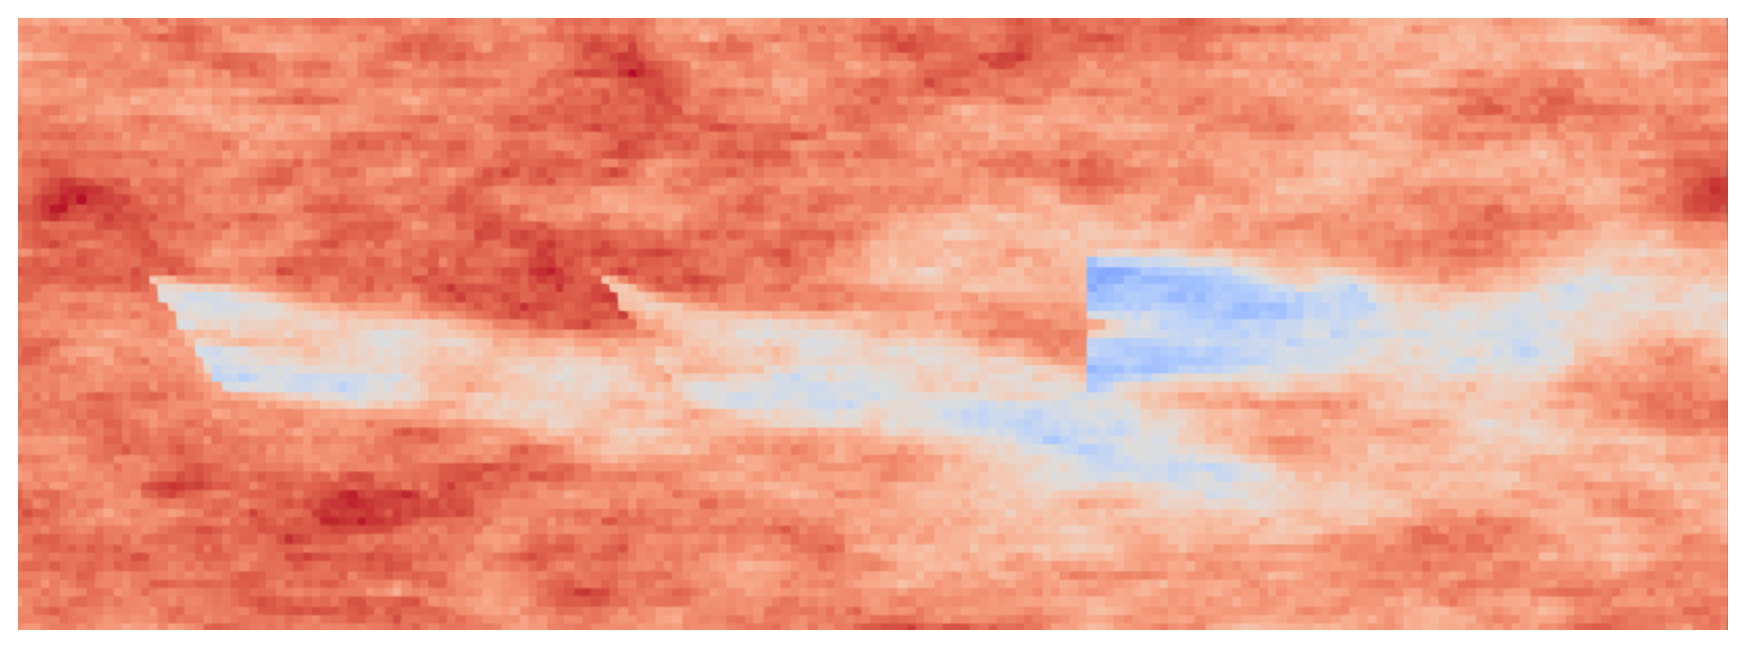
\includegraphics[width=0.6\columnwidth]{figs/simulators/fastfarm_3turb_yawed2.eps}
         \caption{FAST.Farm}
         \label{fig:3turb_fastfarm}
     \end{subfigure}
     % \hfill
\caption[Simulation of our 3-turbines layout on the 2 different simulators, illustrating the difference of fidelity]{Wind velocity field for the simulation of our 3-turbines layout on the 2 simulators: FLORIS and FAST.Farm.}
\end{figure}

Wind farm models serve two main purposes, in the broader literature as in WFCRL. First, when experiments on real wind farms or tunnel experiments on scaled farms are not possible, they are the only way to evaluate
and compare control strategies by predicting their impact on the total power output of a farm. For that purpose, the value of models lie in their accuracy, and the best results are achieved by complex dynamic models involving
costly computations. Secondly, a model of the farm can be used to estimate an optimal command. Here, accuracy must be balanced by tractability, and a constraint on computation time arises for real-time optimization. Of course, evaluating the command on the model used to derive it will likely overestimate its performance: it should rather be evaluated on an other, higher fidelity model which will serve as a substitute for the real farm.

Static models estimate the time-averaged features of the wind flow while ignoring the dynamics of short-term effects, including wake propagation time and wake meandering. They rely on the design of an analytical solution to predict wind speed deficit at a downwind turbine with respect to an upstream turbine  \cite{wake-models}. This gives them the advantage of a very low computation time, as they usually return a solution instantaneously. The wind farm simulation software FLORIS (NREL 2021), created and maintained by the National Renewable Energy Laboratory (NREL), proposes a variety of such models in a single Python framework, and has become a reference for wind farm control engineering. These parametric models combine several components to estimate the effects of turbine yaws on both the redirection of the wake behind the turbine and the velocity in the wake. An example of such a simulation can be found on \Cref{fig:3turb_floris}. 

At higher accuracy and higher computational complexity is FAST.Farm \cite{fast.farm}. It relies on OpenFAST (NREL 2022) to model the dynamics of each individual turbine, but considers additional physics to account for farm-wide ambient wind, as well as wake deficits, propagation dynamics and interactions between different wakes. It supports the implementation of controllers tracking a received yaw reference for each turbine. \Cref{fig:3turb_fastfarm} provides an example of these realistic wind fields. 

FAST.Farm has been shown to be of similar accuracy with high-fidelity large-eddy simulations with much less computational expense. It has been validated against both real wind farm data \cite{shaler2020validation,kretschmer2021fast} and Large Eddy Simulations \cite{fast.farm-validation,shaler2021fast}. Power predictions match real measurements within 2-7\% error on average \cite{shaler2020validation}, although the error can reach 18\% for downstream turbines under low free-stream wind speeds. Load predictions are within 10\% of groundtruth values, with errors reaching 25\% for certain wind directions \cite{shaler2021fast}. Predictions always respect trends in power and load changes: under the same wind conditions, yaws that lead to increases in power output in simulations also lead to increases in real wind farms.

\newpage

\section{Details of the FAST.Farm interface} \label{appendix:interface}

The Python-FAST.Farm interfacing tool relies on two interfaces with \texttt{RECEIVE} and \texttt{SEND} functions. Following \cite{Smits2023interface} in which the authors designed an interface between FAST.Farm and Matlab based on the MPI communication protocol, we rely on an MPI communication channel between the Python and FAST.Farm processes. We choose to let the Python process spawn a new child process to launch the FAST.Farm simulation in the background, allowing the user to only interface with Python. The architecture of the interfacing tool is illustrated in \Cref{fig:fastfarm-interface}.

At every iteration, the FAST.Farm interface retrieves 12 measures per turbine:
\begin{itemize}
    \item 2 wind measurements: wind velocity and direction at the entrance of the farm. The wind direction is estimated by subtracting the yaw estimation error from the current yaw measure.
    \item The current output power of the turbine
    \item The yaw of the turbine
    \item The pitch of the turbine
    \item The torque of the turbine
    \item 6 measures of blade loads: the out-of-plane bending moment estimate for each blade, and the in-plane bending moment estimate on each blade
\end{itemize}

and sends the 3 control targets - yaw, pitch, torque -  to each local turbine controller. Other actuators that are not controlled by the RL algorithm are controlled by the default naive FAST.Farm controllers.


\begin{figure}[!htb]
    \centering
    % \includesvg[width=\columnwidth]{figs/interface/pettingzoo_interface_schema.drawio.svg}
    \def\svgwidth{\columnwidth}
    \import{figs/interface}{pettingzoo_interface_schema_new.pdf_tex}
    \caption{Schema: interfacing infrastructure between FAST.Farm and Python}
    \label{fig:fastfarm-interface}
\end{figure}
Free-stream wind speed and direction are estimated as the wind measurements at the wind turbine with the highest wind speed. Since inflow wind can be turbulent, all estimates are averaged over a period of time defined by the \textit{buffer\_window} parameter.
\newpage

\section{Characteristics of all environments} \label{appendix:envs}
\begin{table}[!htb]
    \centering
    \begin{tabular}{c|c|c}
    \hline
         & \textbf{Centralized Control} & \textbf{Decentralized Control} \\
         \hline
       \textbf{FLORIS}  & \textit{LayoutName\_Floris} & \textit{Dec\_LayoutName\_Floris}\\
       \textbf{FAST.Farm} & \textit{LayoutName\_Fastfarm} & \textit{Dec\_LayoutName\_Fastfarm}\\
       \hline
    \end{tabular}
    \caption{Creating environment IDs: Prefix, Root, Suffix}
    \label{tab:env_id}
\end{table}
For preregistered layouts, every environment is characterized by a tuple of $3$ options, and every environment ID is a combination of the corresponding $3$ parts: a prefix, a root, and a suffix.
\begin{itemize}
    \item The choice to formalize it as a centralized or decentralized control problem. Environments with centralized control are \textit{Gymnasium} environments and expect global actions, i.e. vectors concatenating all actions, and have no prefix. Environments with decentralized control are \textit{PettingZoo} environments and expect local actions sent by each agent. They have the prefix \textit{Dec}.
    \item The choice of the layout, i.e. the arrangement of wind turbines in the field. A list of all layouts is given in \Cref{tab:layoutscharacs}, and a visual overview of them in \Cref{appendix:layouts}. The name of the layout is the root of the environment ID.
    %\md{\\Table 4 is always reffered to as Appendix C, I do not know how to change it.}
    \item The choice of a simulator. Two simulators are for now implemented in WFCRL: the static FLORIS and the dynamic FAST.Farm. The corresponding suffix \textit{Floris} or \textit{Fastfarm} is appended to the environment ID.
\end{itemize}
\begin{table}[!htb] 
\begin{tabular}{ccc}
\hline
\textbf{Layout Name}               & \textbf{\# Agents} & \textbf{Description}       \\
\hline
Ablaincourt                      & 7                  & \begin{tabular}[c]{@{}c@{}}Inspired by layout of the Ablaincourt farm \\ in France, (Duc et al, 2019)\end{tabular}                                        \\
Turb16\_TCRWP                    & 16                 & \begin{tabular}[c]{@{}c@{}}Layout of the Total Control Reference Wind Power Plant \\ (TC RWP) (the first 16 turbines)\end{tabular}                        \\
Turb6\_Row2                      & 6                  & \begin{tabular}[c]{@{}c@{}}Custom case - \\ 2 rows of 6 turbine\end{tabular}                                                                              \\
Turb16\_Row5                     & 16                 & \begin{tabular}[c]{@{}c@{}}Layout of the first 16 turbines in the \\ CL-Windcon project as implemented in WFSim\end{tabular}                              \\
Turb32\_Row5                     & 32                 & \begin{tabular}[c]{@{}c@{}}Layout of the farm used in the \\ CL-Windcon project as implemented in WFSim\end{tabular}                                      \\
TurbX\_Row1 for X in {[}1, 12{]} & X                  & \begin{tabular}[c]{@{}c@{}}Procedurally generated single row layout with X turbines, \\ spaced by 4D with the D the diameter of the turbine.\end{tabular} \\
Ormonde                          & 30                 & Layout of the Ormonde Offshore Wind Farm                                                                                                                  \\
WMR                              & 35                 & Layout of the Westermost Rough Offshore Wind Farm                                                                                                         \\
HornsRev1                        & 80                 & Layout of the Horns Rev 1 Offshore Wind Farm                                                                                                              \\
HornsRev2                        & 91                 & Layout of the Horns Rev 2 Offshore Wind Farm  \\                                                    
\hline                                                        
\end{tabular}
\caption{Preregistered layouts: name, number of agents, and description}
\label{tab:layoutscharacs}
\end{table}



%A visual overview of all layouts is available in \Cref{appendix:layouts}.

\newpage

\section{Environment and Training procedure details}\label{appendix:training-details}

The source code for the WFCRL package is open-sourced under the license Apache v2, and publicly released here \url{www.github.com/ifpen/wfcrl-env}, along with notebook tutorials and documentation.
An example of code snippet allowing the creation of the FLORIS Ablaincourt environment with decentralized control is given below:
\begin{lstlisting}
    from wfcrl import environments as envs
    env = envs.make("Dec_Ablaincourt_Floris")
\end{lstlisting}

The code to reproduce all experiments is available here \url{www.github.com/ifpen/wfcrl-benchmark}. Our algorithm implementations use \textit{PettingZoo}'s Agent Environment Cycle \cite{pettingzoo} interaction logic. Our multi-agent environments also support standard \textit{Gymnasium}-like RL control loops via the \textit{PettingZoo}'s \texttt{aec\_to\_parallel} function.

We report in \Cref{tab:parameters-ppo} the hyper-parameters used for IPPO and MAPPO, and in \Cref{tab:parameters-dqn} the hyper-parameters used for QMIX and IDRQN. Recurrent Q-networks in QMIX and IDRQN take as input both the current local observation and the last action taken by the agent. All algorithms are trained on episodes of length $T=150$ (\textit{Sc. 1}) or $T=2048$ (\textit{Sc. 2}) with $\beta = 0.99$. Evaluation is done on episodes of length $T=150$. 
\begin{table}[!htb]
    \centering
    \begin{tabular}{c|c}
    \hline
    \textbf{Parameter} & \textbf{Value}\\
    %\bottomrule \\
    \hline
    Learning rate & 0.0003 $\rightarrow$ 0 (linear annealing) \\
    $\beta$ & 0.99\\
    GAE $\lambda$ & 0.95\\
    \# minibatches & 32\\
    \# epochs & 10\\
    Normalize advantages & True\\
    Clip coefficient & 0.2\\
    Value loss coefficient & 0.5\\
    Maximum gradient norm & 0.5\\
    Hidden layers & (64, 64)\\
    \# steps between updates & 2048\\
    Batch size & 2048\\
    Minibatch size & 64\\
    % \# iterations & 24\\
    \hline
    \end{tabular}
    \caption{PPO Experiment hyperparameters (used in IPPO and MAPPO)}
    \label{tab:parameters-ppo}
\end{table}

\begin{table}[!htb]
    \centering
    \begin{tabular}{c|c}
    \hline
    \textbf{Parameter} & \textbf{Value}\\
    %\bottomrule \\
    \hline
    & \\
    \textit{Shared parameters (Q-networks)} & \\
    & \\
    Learning rate & 0.0005 \\
    $\beta$ & 0.99\\
    Hidden layers & 64 \\
    \# layers & 2 \\
    Batch size (episodes) & 32\\
    Buffer size (episodes) & 200 \\
    Exploration $\epsilon$ & 1 $\rightarrow$ 0.05 \\
    Target network frequency (episodes) & 25 \\ 
    % \# iterations & 24\\
    $i$th Q-Network input& ($o^i_t, a^i_{t-1})$\\
    \hline
    & \\
    \textit{QMIX Hypernetwork Parameters} \\
    & \\
    % \hline
     Hidden layer dim & 32 \\
     \# layers & 2
    \end{tabular}
    \caption{QMIX and IDRQN (Independent DQN with deep recurrent network) experiment hyperparameters}
    \label{tab:parameters-dqn}
\end{table}


%tau: 1.0

% \begin{table}[!htb]
%     \centering
%     \begin{tabular}{c|cc}
%     & \textbf{IPPO} & \textbf{MAPPO}\\
%     \bottomrule \\
%     % seed & 1 & \\
%     % torch\_deterministic & True & \\
%     % cuda & True & \\
%     % track & True & \\
%     % wandb\_entity & None & \\
%     % save\_model & True & \\
%     % total\_timesteps & 50000 & \\
%     learning\_rate & 0.0003 & \\
%     gamma & 0.99 & \\
%     gae\_lambda & 0.95 & \\
%     num\_minibatches & 32 & \\
%     update\_epochs & 10 & \\
%     norm\_adv & True & \\
%     clip\_coef & 0.2 & \\
%     clip\_vloss & True & \\
%     ent\_coef & 0.0 & \\
%     vf\_coef & 0.5 & \\
%     max\_grad\_norm & 0.5 & \\
%     target\_kl & None & \\
%     % num\_envs & 1 & \\
%     % no\_reset & False & \\
%     kl\_coef & 0.0 & \\
%     % policy & base & \\
%     % adaptive\_explo & False & \\
%     % multi\_scale & False & \\
%     hidden\_layer\_nn & (64, 64) & \\
%     % debug & False & \\
%     num\_steps & 2048 & \\
%     anneal\_lr & True & \\
%     batch\_size & 2048 & \\
%     minibatch\_size & 64 & \\
%     num\_iterations & 24 & \\
%     % num\_agents & 1 & \\
%     % reward\_shaping &  & \\
%     \end{tabular}
%     \caption{Experiment Hyperparameters}
%     \label{tab:fastfarm_eval}
% \end{table}

The experiments were run on $3$ different computers. The first computer, which has no GPU and a Intel Xeon Gold 6240Y processor, was used to train IPPO and MAPPO on \textit{Wind Scenario I} for $1$ week of compute. On the second computer, an internal cluster with a GPU Quadro RTX 6000 24Go, $2$ week of compute was used to to train experiments of \textit{Wind Scenario II}. The last computer which has a Intel Xeon Gold 6240Y processor was used for training models during $3$ days of compute on \textit{Wind Scenario I}, and for evaluation purposes.
%
%1 [machine ifpen details] + 1 [machine CLEPS details.]
%
\newpage

\section{Score: wind rose and weights}

In this section we illustrate the use of wind statistics from the SMARTEOLE dataset to extract wind conditions weights $\rho$ of the evaluation score \eqref{eq:eval_eq}. In \Cref{fig:windrose}, we report the distribution of wind velocity and direction in the SMARTEOLE dataset. In \Cref{fig:smarteole-weights}, we show the corresponding extracted weights $\rho$ for the $25$ corresponding wind conditions.

\begin{figure}[!htb]
    \centering
    \begin{subfigure}{0.4\columnwidth}
        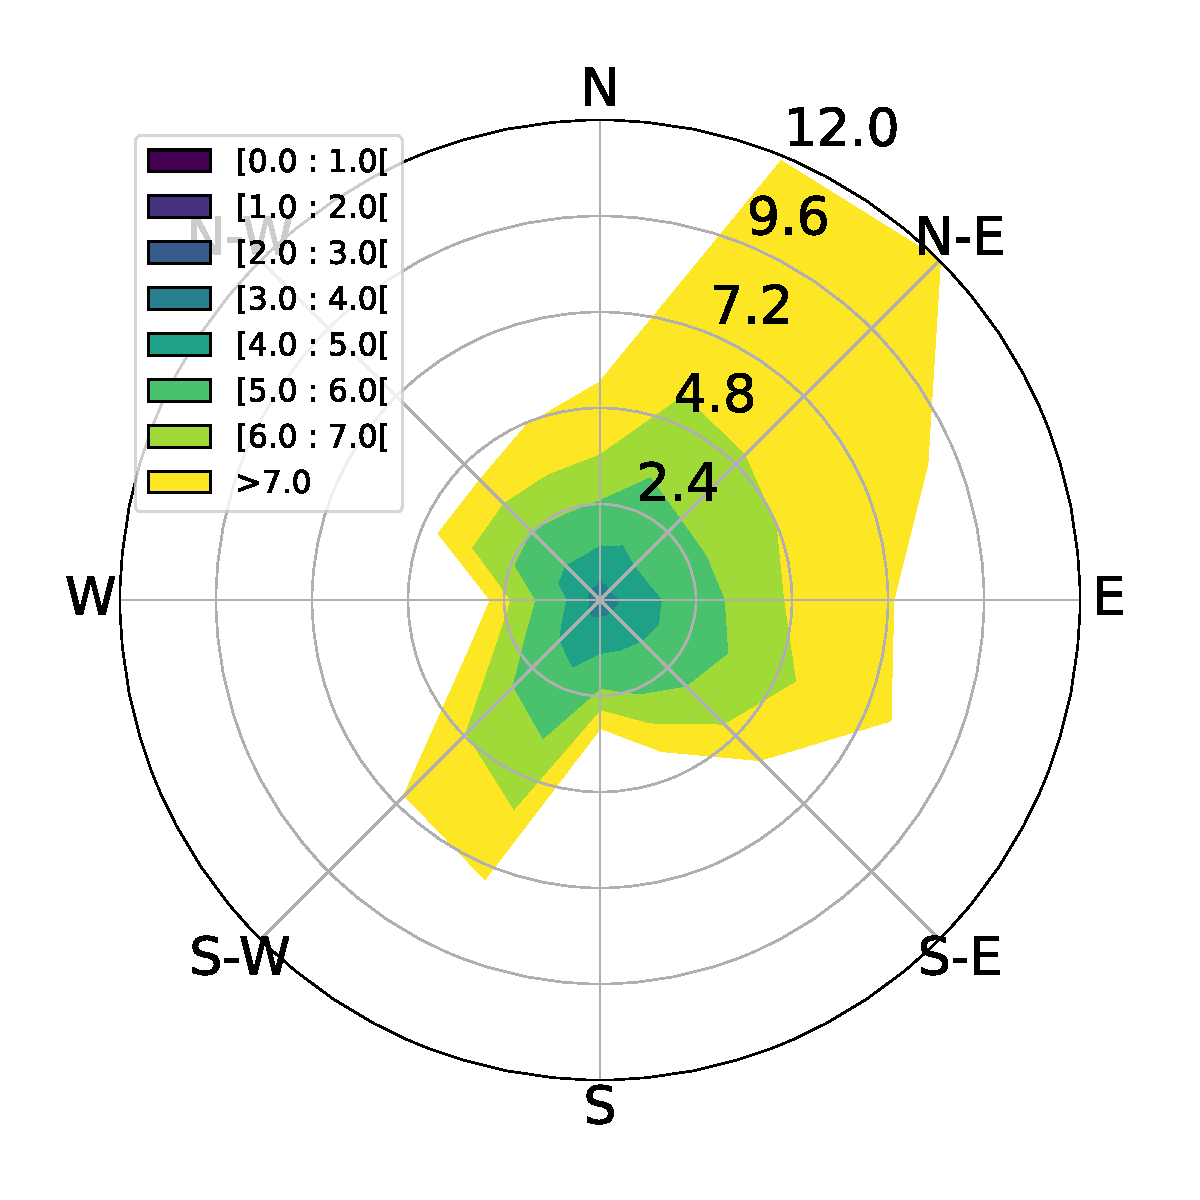
\includegraphics[width=\columnwidth]{figs/windrose/windrose_smarteole2.pdf}
        % \includesvg[width=\columnwidth]{figs/windrose/windrose_smarteole2.svg}
    \caption{Wind conditions in SMARTEOLE}
    \label{fig:windrose}
    \end{subfigure}
    \begin{subfigure}{0.55\columnwidth}
     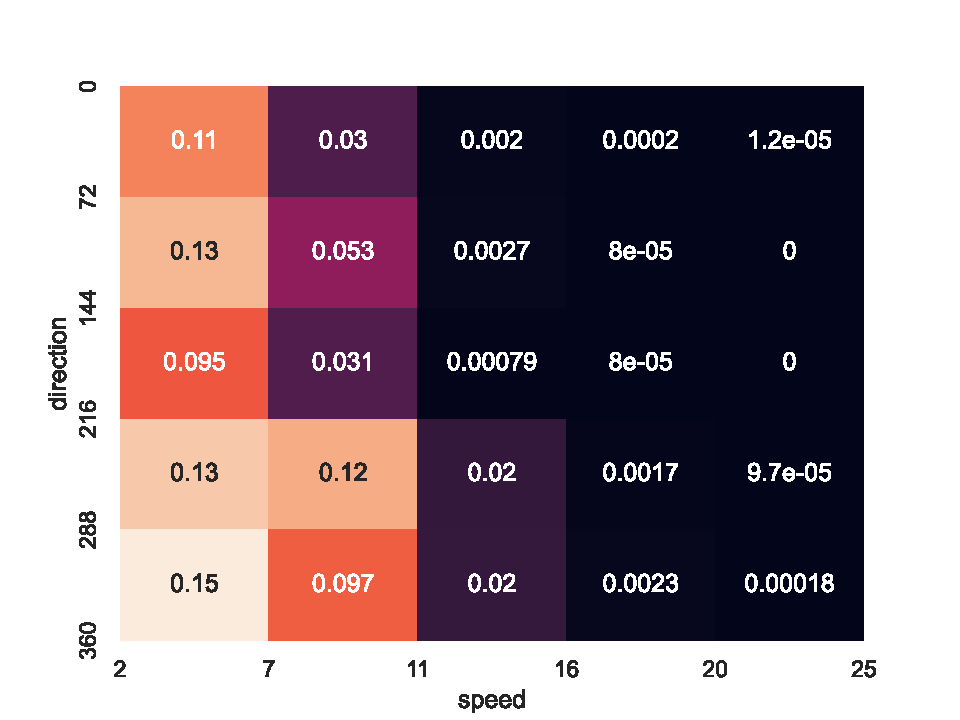
\includegraphics[width=\columnwidth]{figs/windrose/windrose_weights2.pdf}
    %  \includesvg[width=\columnwidth]{figs/windrose/windrose_weights2.svg}
     \caption{$\rho_i$ extracted from SMARTEOLE}
     \label{fig:smarteole-weights}
     \end{subfigure}
     \caption{Extraction of the $\rho_i$ weights from the SMARTEOLE dataset. The empirical distribution of wind speed and direction in the data represented as a windrose is in (a), and the corresponding extracted weights $\rho_i$ given to each of the $25$ wind conditions are in (b).}
\end{figure}

\newpage

\section{More benchmark results}\label{appendix:results}
\subsection{Evaluation and transfer on FAST.Farm}\label{appendix:transfer-curves}
%\md{We report the results on the FAST.Farm evaluation task in \Cref{tab:fastfarm_eval}.} 
The literature on transferring wind farm control policies from lower to higher fidelity simulators is scarce. In \cite{monroc2024towards}, a transfer method is proposed that relies on a complex combination of optimization in static models, supervised learning of policies, policy evaluation and problem-specific reward engineering. The development of simpler transfer solutions that are less problem-dependent will be necessary to progress towards the deployment of RL policies on real wind farms. Yet as we show here, a naive fine-tuning approach might not be enough. 
%We evaluate the agents trained on the FLORIS environments by rolling out their determinist policies in this new environment (they always pick the likeliest action under their policy functions). 
On this task, we simulate a $900$ steps episode of the \textit{Turb3Row1} layout on FAST.Farm (environment  \textit{Dec\_Turb3\_Row1\_Fastfarm}). 
%The average rewards collected during the episode are in \Cref{tab:fastfarm_eval}. 

For the \textit{Transfer} task, we pursue the training in the new environments, and report the evolution of the power and load compared to the \textit{Eval} case in \Cref{fig:transfer-curves} for the agents trained under IPPO. We simulate a day of training on FAST.Farm, correponding to $28800$ steps in the environment.  
%
\begin{figure}[!htb]
    \centering
    \centering
     \begin{subfigure}{0.45\columnwidth}
     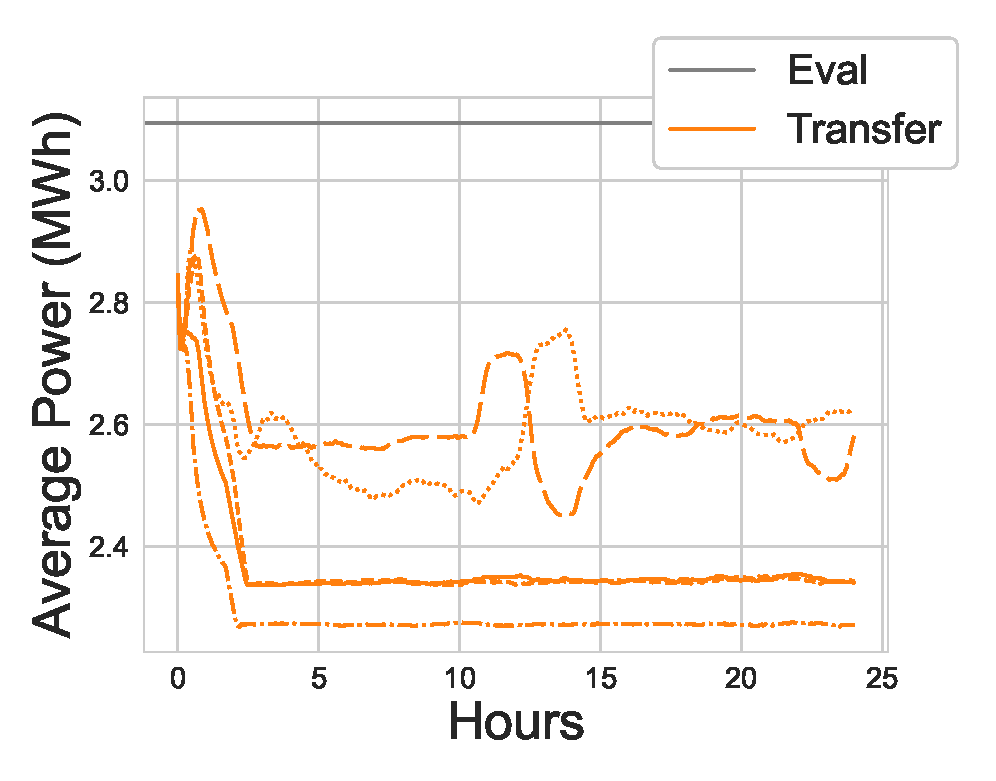
\includegraphics[width=\columnwidth]{figs/xps_turb3/transfer/power_transfer.eps}
     \caption{Power}
    \end{subfigure}
     \begin{subfigure}{0.45\columnwidth}
     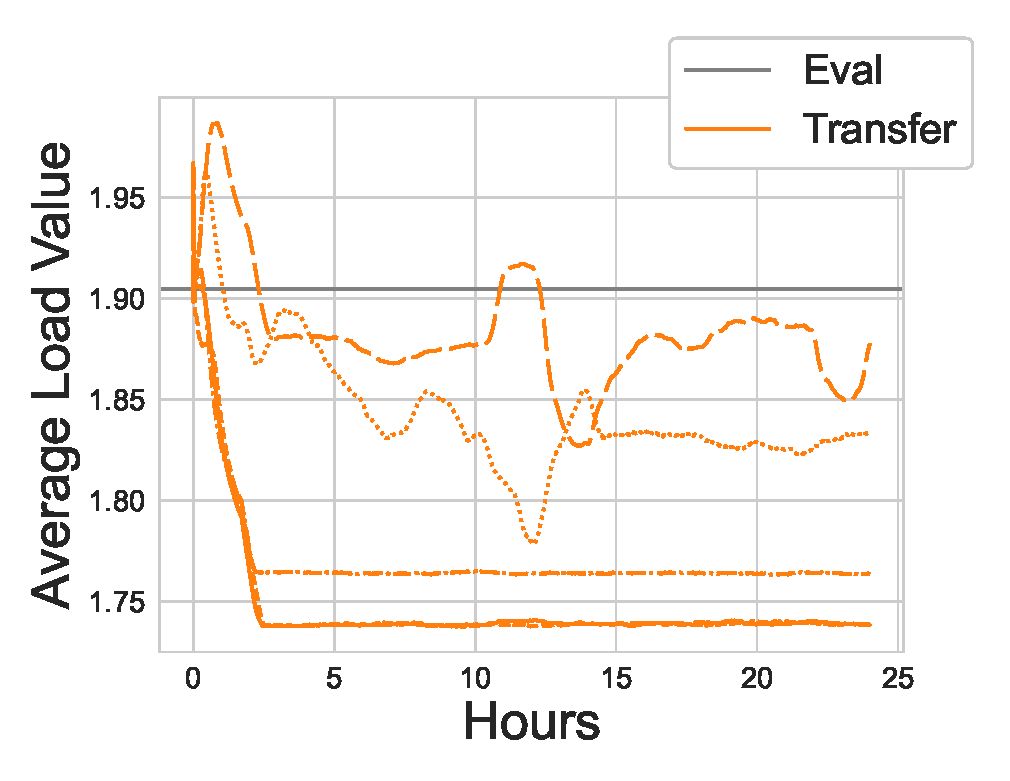
\includegraphics[width=\columnwidth]{figs/xps_turb3/transfer/load_transfer.eps}
     \caption{Load}
     \end{subfigure}
     \caption{Evaluation and transfer on FAST.Farm: evolution of power (left) and load (right) on the \textit{Dec\_Turb3\_Row1\_Fastfarm} environment. Results are reported for $5$ seeds.}
    \label{fig:transfer-curves}
\end{figure}
%
% \begin{table}[!htb]
%     \centering
%     \begin{tabular}{c|cc}
%     \hline
%     & \textbf{IPPO} & \textbf{MAPPO}\\
%     %\bottomrule \\
%     \hline
%        \textit{Turb3Row1 (Sc. 1)}  & $1238	\pm 24$
%         & $1369 \pm 41$  \\
%         \textit{Turb3Row1 (Sc. 2)} & $1607 \pm	41$ &	$1369	\pm 124$ \\
%         \hline
%     \end{tabular}
%     \caption{FAST.Farm evaluation task}
%     \label{tab:fastfarm_eval}
% \end{table}
%
During the evaluation tasks, policies learned on FLORIS (IPPO, \textit{Sc. I}) deployed on the dynamic simulator achieve an increase of 15\% in power production over the baseline. We know from existing literature that on \textit{Turb3Row1}, there exists a policy that reaches an increase of 21\% \cite{monroc2024towards}. The difference in performance suggests that we could benefit from further fine-tuning these policies on the dynamic simulation. However, the simple transfer learning strategy pursued during the \textit{Transfer} task degrades the performance of the policies when learning online, reaching an average of 0\% increase over the greedy baseline at the end of the experiments. This illustrates the challenge of designing robust methods to bridge the gap between simple simulators and complex real world dynamics. 

\subsection{More training results}
In this section we report more benchmark results. The training curves of IPPO and MAPPO (resp. QMIX and IDRQN) under \textit{Wind Scenario I} on the \textit{Turb3Row1} layout are in \Cref{fig:turb3-wfixed-results} (resp \Cref{fig:turb3-wfixed-results-valuebase}). As the latter, value-based algorithms require a discretization of the action space, we report their results separately. We use an action space of $3$ actions: increase actuation target value, decrease it, or do nothing. Each change in actuation leads to a change of $5\degree$ in the actuation space. \Cref{tab:train_scores} summarizes the evaluation scores, reporting mean and standard deviation on the $5$ seeds. 

%on all tasks at convergence: 
%both on the total score and the increase or decrease in average power of load compared to the greedy baseline, for both the  \textit{Turb3Row1} and  \textit{Ablaincourt} layouts. 

\begin{figure}[!htb]
     \centering
     \begin{subfigure}{0.32\columnwidth}
     
\includegraphics[width=\columnwidth]{figs/wfixed/reward/Turb3_Row1_Floris_constant_score.eps}
     \caption{Episode Reward}
     \end{subfigure}
     \begin{subfigure}{0.32\columnwidth}
     
\includegraphics[width=\columnwidth]{figs/wfixed/powers/Turb3_Row1_Floris_constant_score.eps}
     \caption{Episode Power Output}
     \end{subfigure}
     \begin{subfigure}{0.32\columnwidth}
     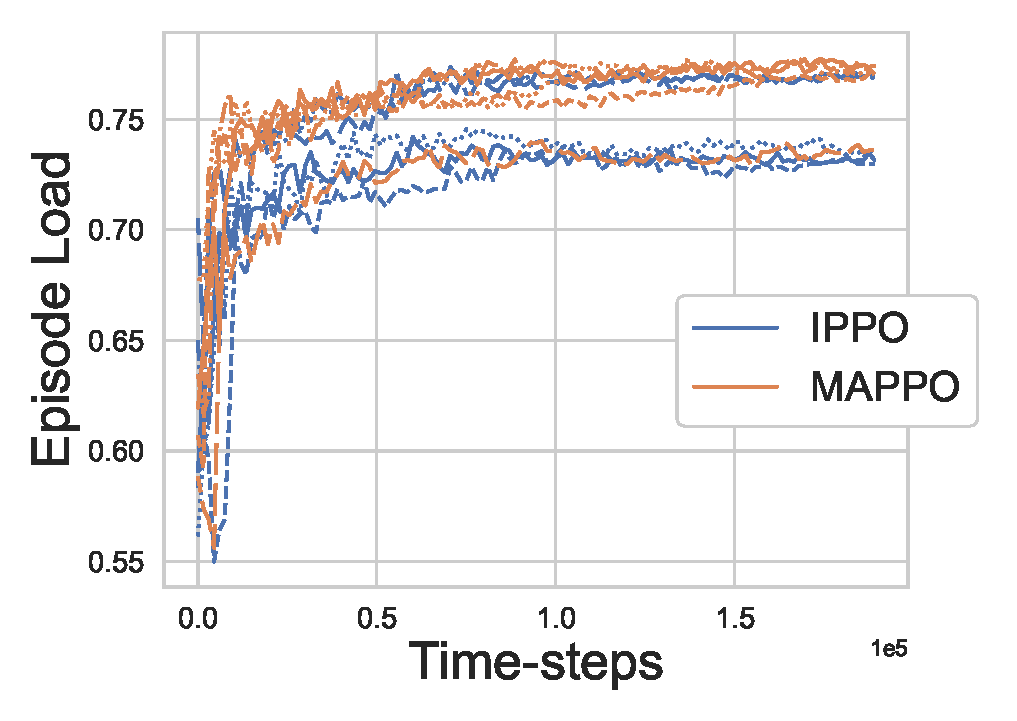
\includegraphics[width=\columnwidth]{figs/wfixed/loads/Turb3_Row1_Floris_constant_score.eps}
     \caption{Episode Load Indicator}
     \end{subfigure}
     \begin{subfigure}{0.32\columnwidth}
     
\includegraphics[width=\columnwidth]{figs/wfixed/reward/Ablaincourt_Floris_constant_score.eps}
     \end{subfigure}
     \begin{subfigure}{0.32\columnwidth}
     
\includegraphics[width=\columnwidth]{figs/wfixed/powers/Ablaincourt_Floris_constant_score.eps}
     \end{subfigure}
     \begin{subfigure}{0.32\columnwidth}
     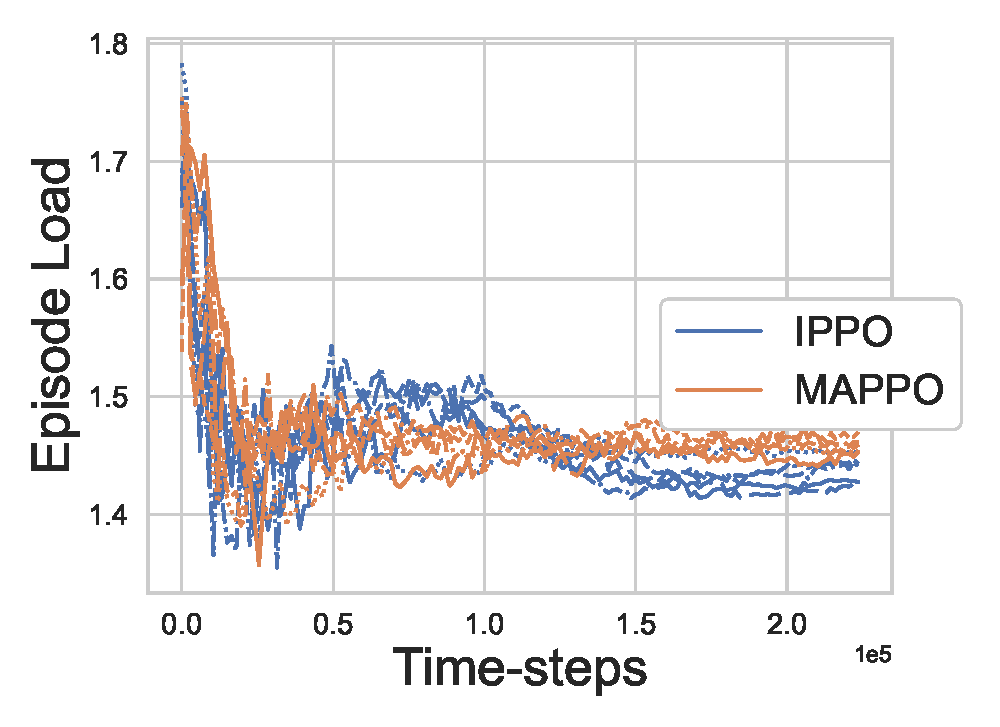
\includegraphics[width=\columnwidth]{figs/wfixed/loads/Ablaincourt_Floris_constant_score.eps}
     \end{subfigure}
\caption{Evolution of episode reward (a), power output (b) and load indicator (c) on the layout \textit{Turb3Row1} (top) and \textit{Ablaincourt} (down) FLORIS environments for actor-critic algorithms IPPO and MAPPO during training. Deterministic policies are evaluated every $5$ training steps.}
 \label{fig:turb3-wfixed-results}
\end{figure}

\begin{figure}[!htb]
     \centering
     \begin{subfigure}{0.32\columnwidth}
     
\includegraphics[width=\columnwidth]{figs/wfixed/reward/value-based/Turb3_Row1_Floris_constant_score.eps}
     \caption{Episode Reward}
     \end{subfigure}
     \begin{subfigure}{0.32\columnwidth}
     
\includegraphics[width=\columnwidth]{figs/wfixed/powers/value-based/Turb3_Row1_Floris_constant_score.eps}
     \caption{Episode Power Output}
     \end{subfigure}
     \begin{subfigure}{0.32\columnwidth}
     
\includegraphics[width=\columnwidth]{figs/wfixed/loads/value-based/Turb3_Row1_Floris_constant_score.eps}
     \caption{Episode Load Indicator}
     \end{subfigure}
     \begin{subfigure}{0.32\columnwidth}
     
\includegraphics[width=\columnwidth]{figs/wfixed/reward/value-based/Ablaincourt_Floris_constant_score.eps}
     \end{subfigure}
     \begin{subfigure}{0.32\columnwidth}
     
\includegraphics[width=\columnwidth]{figs/wfixed/powers/value-based/Ablaincourt_Floris_constant_score.eps}
     \end{subfigure}
     \begin{subfigure}{0.32\columnwidth}
     
\includegraphics[width=\columnwidth]{figs/wfixed/loads/value-based/Ablaincourt_Floris_constant_score.eps}
     \end{subfigure}
\caption{Evolution of episode reward (a), power output (b) and load indicator (c) on \textit{Turb3Row1} (top) and \textit{Ablaincourt} (down) FLORIS environments during training. Value-based approaches QMIX and IDRQN. Deterministic policies are evaluated every $50$ episodes.}
 \label{fig:turb3-wfixed-results-valuebase}
\end{figure}

\begin{table}[!htb]
\ra{1.2}
\centering
\begin{tabular}{lllllll}
\multicolumn{1}{c}{} & & & & & & \\
% & & \multicolumn{6}{c}{Evaluation Task} \\
\multicolumn{1}{c}{} & \multicolumn{3}{c}{\textbf{Turb3Row1}} & \multicolumn{3}{c}{\textbf{Ablaincourt}} \\
\hline
\multicolumn{1}{c}{}& \multicolumn{2}{c}{\textbf{FLORIS}} & \textbf{FAST.Farm}& \multicolumn{2}{c}{\textbf{FLORIS}} & \textbf{FAST.Farm}\\
\hline
& \textit{Sc. 1} & \textit{Sc. 2} & \textit{Sc. 1}  & \textit{Sc. 1} & \textit{Sc. 2} & \textit{Sc. 1}\\
\hline
& & & & & &  \\
\multicolumn{7}{c}{Training on \textit{Sc. 1}} \\
& & & & & &  \\
%& & Turb3\_Row1\_Floris\_constant & Turb3\_Row1\_Floris\_windrose & Turb3\_Row1\_Fastfarm\_constant & Ablaincourt\_Floris\_constant & Ablaincourt\_Floris\_windrose & Ablaincourt\_Fastfarm\_constant \\
IPPO & \textbf{239.5} $\pm$ 2.4 & 354.8 $\pm$ 14.4 & 217.4 $\pm$ 1.8 & 351.0 $\pm$ 0.3 & 329.9 $\pm$ 1.4 & 327.4 $\pm$ 1.6 \\
 MAPPO & 237.7 $\pm$ 2.1 & 345.1 $\pm$ 12.6 & 215.3 $\pm$ 1.4 & \textbf{351.7} $\pm$ 0.1 & 327.6 $\pm$ 1.4 & \textbf{330.2} $\pm$ 0.1 \\
IDQN & 202.6 $\pm$ 21.5 & 278.8 $\pm$ 31.8 & 173.5 $\pm$ 28.7 & 263.3 $\pm$ 11.2 & 231.4 $\pm$ 7.9 & 189.3 $\pm$ 10.5 \\
IDRQN & 210.6 $\pm$ 20.7 & 295.1 $\pm$ 32.2 & 184.8 $\pm$ 28.7 & 257.1 $\pm$ 2.5 & 240.8 $\pm$ 3.5 & 183.0 $\pm$ 0.6 \\
QMIX & 193.5 $\pm$ 17.0 & 273.1 $\pm$ 26.3 & 161.0 $\pm$ 23.4 & 254.8 $\pm$ 0.7 & 230.8 $\pm$ 11.1 & 181.7 $\pm$ 0.2 \\
& & & & & & \\
\hline
& & & & & & \\
\multicolumn{7}{c}{Training on \textit{Sc. 2}} \\
& & & & & & \\
% \hline
 IPPO & 203.7 $\pm$ 4.3 & \textbf{406.0} $\pm$ 10.5& \textbf{218.7} $\pm$ 0.5 & 321.8 $\pm$ 7.5 & \textbf{354.6} $\pm$ 4.1  & 317.3 $\pm$ 4.1 \\
MAPPO & 213.7 $\pm$ 10.2 & 372.4 $\pm$ 15.5 & 218.0 $\pm$ 1.0 & 329.2 $\pm$ 11.0 & 314.6 $\pm$ 3.4 & 319.8 $\pm$ 3.7 \\
IDQN & 193.8 $\pm$ 17.0 & 262.0 $\pm$ 10.1 & 161.7 $\pm$ 22.9 & 263.1 $\pm$ 4.8 & 230.5 $\pm$ 8.2 & 197.7 $\pm$ 12.0 \\
IDRQN & 199.1 $\pm$ 16.8 & 343.7 $\pm$ 52.4 & 189.7 $\pm$ 24.5 & 299.0 $\pm$ 7.5 & 276.9 $\pm$ 11.6 & 249.2 $\pm$ 13.5 \\
QMIX & 200.9 $\pm$ 18.1 & 313.4 $\pm$ 50.6 & 180.5 $\pm$ 28.7 & 262.3 $\pm$ 14.3 & 245.9 $\pm$ 25.9 & 189.2 $\pm$ 10.4
\end{tabular}
\caption{Results at the end of training, on $200k$ and $2M$ time-steps for \textit{Turb3Row1} and \textit{Ablaincourt} respectively. \textit{Sc. 1} (resp \textit{Sc. 2}) corresponds to the firts Wind Scenario I (resp. II). All models are evaluated on both scenarios. For a decomposition in power and load penalty contribution, see \Cref{tab:train_loads} and \Cref{tab:train_powers}.} \label{tab:train_scores}
\end{table} 

We also report for the evaluated models on \textit{Sc. I} the decomposition of the episode reward in power output (\Cref{tab:train_powers}) and load penalty (\Cref{tab:train_loads}). \Cref{tab:train_powers} is equivalent to the total energy produced during the episode, while \Cref{tab:train_loads} can be interpreted as an indication of accumulated damage. An example of a the rollout of a policies learned with IPPO on Scenario I is given in \Cref{fig:qualit-policies} for \textit{Turb3Row1} and \textit{Ablaincourt}. In both layouts, the wake of the last turbine in the row has no impact on the production of the others. Its rotor is therefore maintained facing the wind, as in the greedy solution (yaw of $0\degree$). On \textit{Turb3Row1}, where a row of $3$ turbines are perfectly aligned with the wind direction, learned policies alternatively lead the yaws of the first turbines to around $+30\degree$ or $-30\degree$. On \textit{Ablaincourt} on the other hand, learned policies always converge towards negative yaws.
 
\begin{table}[!htb]
\ra{1.2}
\centering
\begin{tabular}{lllll}
 & \multicolumn{2}{c}{\textbf{Turb3Row1}} & \multicolumn{2}{c}{\textbf{Ablaincourt}} \\
\hline
 & \multicolumn{1}{c}{\textbf{FLORIS}} & \textbf{FAST.Farm}& \multicolumn{1}{c}{\textbf{FLORIS}} & \textbf{FAST.Farm}\\
 \hline
& & & & \\
\multicolumn{5}{c}{Training on \textit{Sc. 1}} \\
& & & & \\
IPPO & 190.3 $\pm$ 2.0 & 239.6 $\pm$ 1.0 & 222.6 $\pm$ 5.4 & 245.0 $\pm$ 0.8 \\
MAPPO & 194.3 $\pm$ 1.9 & 237.5 $\pm$ 0.5 & 218.6 $\pm$ 5.8 & 239.8 $\pm$ 1.5 \\
IDQN & 159.1 $\pm$ 1.0 & 128.3 $\pm$ 0.7 & 157.6 $\pm$ 1.7 & 126.8 $\pm$ 1.7 \\
IDRQN & 160.5 $\pm$ 5.7 & 129.0 $\pm$ 4.7 & 168.1 $\pm$ 22.6 & 126.8 $\pm$ 1.2 \\
QMIX & 159.6 $\pm$ 2.2 & 128.7 $\pm$ 2.1 & 157.0 $\pm$ 0.5 & 126.3 $\pm$ 0.5 \\
\hline
& & & &  \\
\multicolumn{5}{c}{Training on \textit{Sc. 2}} \\
& & & & \\
IPPO & \textbf{247.1} $\pm$ 7.1 & \textbf{251.6} $\pm$ 2.7 & \textbf{251.4} $\pm$ 0.5 & \textbf{253.4} $\pm$ 0.8 \\
MAPPO & 219.0 $\pm$ 32.7 & 248.8 $\pm$ 2.5 & 224.8 $\pm$ 20.5 & 247.6 $\pm$ 0.3 \\
IDQN & 159.6 $\pm$ 0.0 & 128.7 $\pm$ 0.0 & 159.4 $\pm$ 0.5 & 128.3 $\pm$ 0.7 \\
IDRQN & 176.1 $\pm$ 38.0 & 151.2 $\pm$ 51.6 & 176.2 $\pm$ 37.9 & 152.0 $\pm$ 51.2 \\
QMIX & 196.6 $\pm$ 45.2 & 179.3 $\pm$ 61.3 & 177.3 $\pm$ 36.5 & 127.6 $\pm$ 1.1
\end{tabular}
\caption{Sum of total power output at every time-step for an evaluation episode with constant wind conditions (\textit{Sc. 1})  at the end of training, after $200k$ time-steps for \textit{Turb3Row1} and $2M$ time-steps for \textit{Ablaincourt}.} 
\label{tab:train_powers}
\end{table}


\begin{table}[!htb]
\ra{1.2}
\centering
\begin{tabular}{lllll}
 & \multicolumn{2}{c}{\textbf{Turb3Row1}} & \multicolumn{2}{c}{\textbf{Ablaincourt}} \\
\hline
 & \multicolumn{1}{c}{\textbf{FLORIS}} & \textbf{FAST.Farm}& \multicolumn{1}{c}{\textbf{FLORIS}} & \textbf{FAST.Farm}\\
 \hline
& & & & \\
\multicolumn{5}{c}{Training on \textit{Sc. 1}} \\
& & & & \\
 %& Turb3\_Row1\_Floris & Turb3\_Row1\_Fastfarm & Ablaincourt\_Floris & Ablaincourt\_Fastfarm \\
IPPO & 84.0 $\pm$ 0.9 & 343.6 $\pm$ 3.4 & 82.3 $\pm$ 1.0 & 350.5 $\pm$ 0.5 \\
MAPPO & 84.7 $\pm$ 0.7 & 345.5 $\pm$ 2.9 & 82.9 $\pm$ 0.8 & 348.3 $\pm$ 0.8 \\
IDQN & 83.9 $\pm$ 0.1 & \textbf{285.7} $\pm$ 0.4 & 84.0 $\pm$ 0.2 & 284.9 $\pm$ 0.9 \\
IDRQN & 83.7 $\pm$ 0.6 & 286.1 $\pm$ 2.5 & 84.0 $\pm$ 0.2 & 284.9 $\pm$ 0.6 \\
QMIX & 83.8 $\pm$ 0.2 & 285.9 $\pm$ 1.1 & 84.1 $\pm$ 0.0 & \textbf{284.7} $\pm$ 0.3 \\
\hline
& & & &  \\
\multicolumn{5}{c}{Training on \textit{Sc. 2}} \\
& & & & \\
IPPO & \textbf{75.5} $\pm$ 2.2 & 351.7 $\pm$ 2.0 & \textbf{74.2} $\pm$ 0.3 & 352.5 $\pm$ 0.8 \\
MAPPO & 78.6 $\pm$ 3.2 & 349.5 $\pm$ 2.3 & 79.1 $\pm$ 2.1 & 350.6 $\pm$ 2.1 \\
%IDQN & 83.8 $\pm$ nan & 285.9 $\pm$ 0.0 & 83.9 $\pm$ 0.0 & 285.7 $\pm$ 0.4 \\
IDRQN & 82.0 $\pm$ 4.1 & 297.9 $\pm$ 27.5 & 82.0 $\pm$ 4.1 & 298.3 $\pm$ 27.3 \\
QMIX & 79.8 $\pm$ 4.9 & 312.8 $\pm$ 32.7 & 82.0 $\pm$ 3.7 & 285.4 $\pm$ 0.6
\end{tabular}
\caption{Sum of load penalties for an evaluation episode with constant wind conditions (\textit{Sc. 1}) after $200k$ time-steps for \textit{Turb3Row1} and $2M$ time-steps for \textit{Ablaincourt}.} \label{tab:train_loads}
\end{table}

% \begin{table}[!htb]
%     \centering
%     \begin{tabular}{c|ccc|ccc}
%     \hline
%     & \multicolumn{3}{c}{\textbf{IPPO}} & \multicolumn{3}{c}{\textbf{MAPPO}} \\
%     %\bottomrule \\
%     \hline
%     & Score & Power (\%) & Load (\%) & Score & Power (\%) & Load (\%) \\
%     %\bottomrule \\
%     \hline
%        \textit{Turb3. (Sc. 1)}  & $\textbf{3431} \pm \textbf{138}$	& $+18  \pm	5$ & $	+30 	\pm 11$ &	$3362 \pm	135$	& $+15 \pm	5$ & $	+27 \pm	12$ \\
%  \textit{Turb3. (Sc. 2)}  & $\textbf{5501}	\pm \textbf{86}$	& -& - &	$4757 \pm 164$	& - & - \\
%         \textit{Abl. (Sc. 1)} & $3968	\pm 29$ &	$+5  \pm	1	$ & $-15	\pm 2$ &	$\textbf{4035}	\pm \textbf{7}$ & 	$+7 \pm 0.3$ & $-16 \pm	3$ \\
%         \textit{Abl. (Sc. 2)} & $\textbf{4430} \pm	\textbf{22}$ &	- & - &	$3808 \pm	275$ & 	- & - \\
% \hline
%     \end{tabular}
%     \caption{Results at the end of training IPPO and MAPPO, on $50k$ and $500k$ time-steps for \textit{Turb3Row1} (\textit{Turb3.} in the table ) and \textit{Ablaincourt} (\textit{Abl.} in the table) respectively. \textit{Sc. 1} (resp \textit{Sc. 2}) corresponds to the firts Wind Scenario I (resp. II).}
%     \label{tab:train_scores}
% \end{table}

\begin{figure}
    \centering
    \begin{subfigure}{1\columnwidth}
        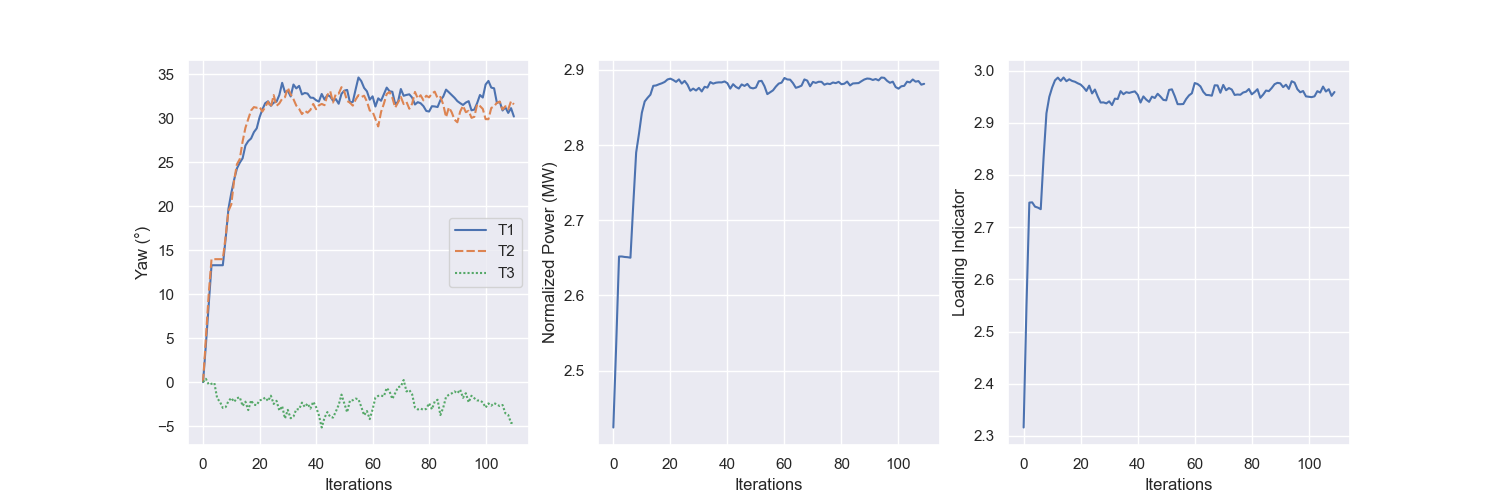
\includegraphics[width=\linewidth]{figs/wfixed/behavior/plot0.png}
    \end{subfigure}
    \begin{subfigure}{1\columnwidth}
        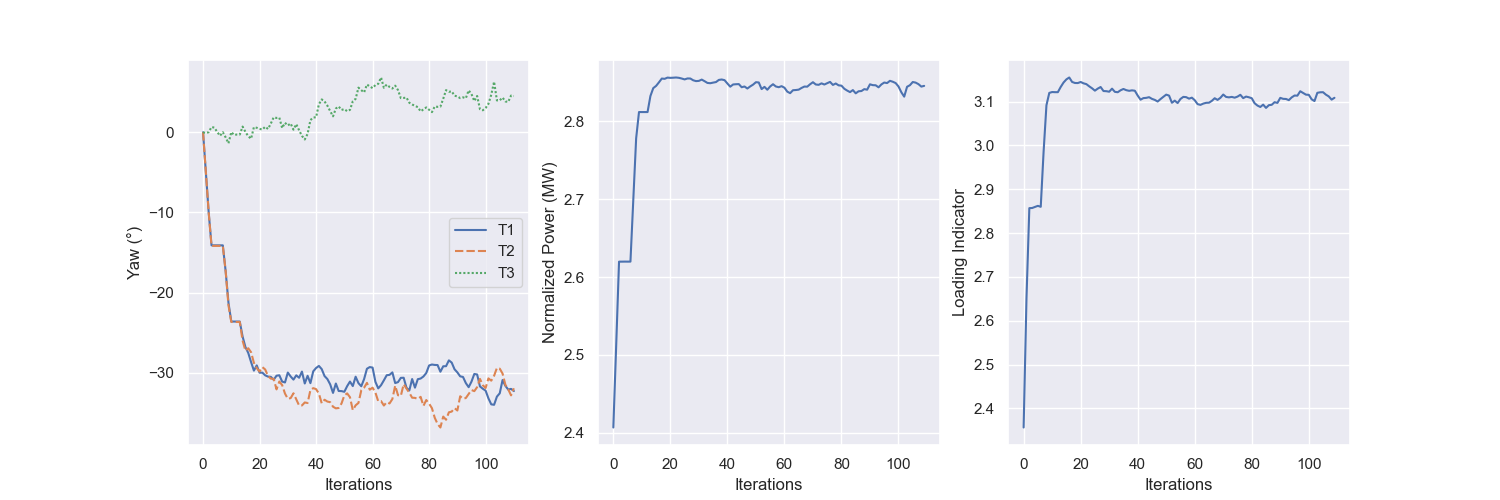
\includegraphics[width=\linewidth]{figs/wfixed/behavior/plot.png}
    \end{subfigure}
    \begin{subfigure}{1\columnwidth}
        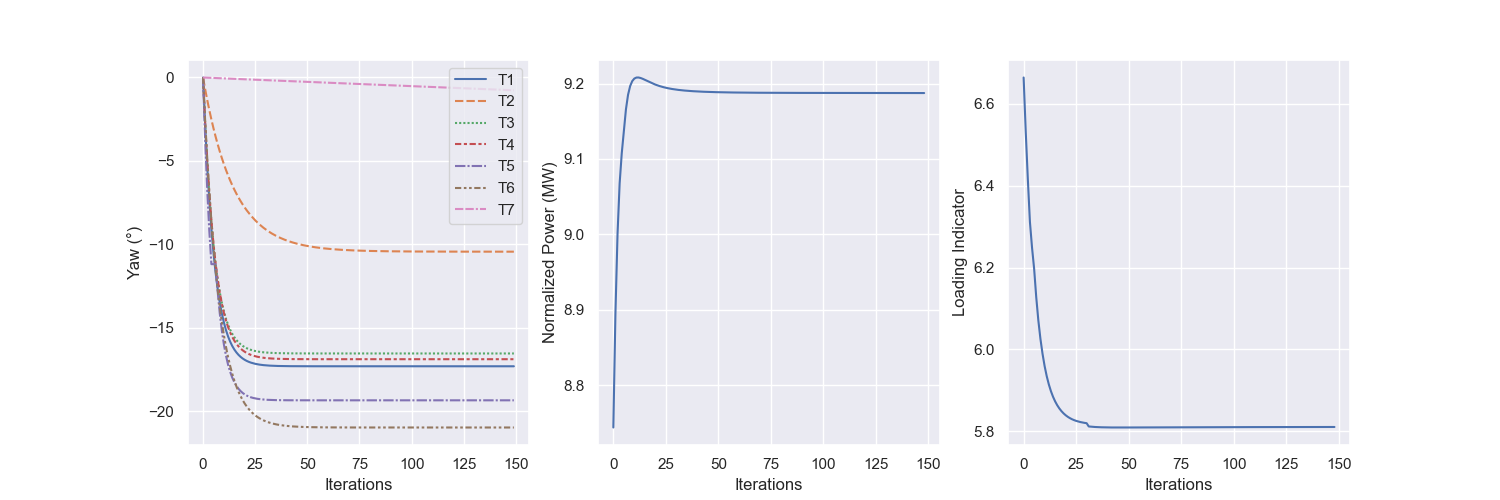
\includegraphics[width=\linewidth]{figs/wfixed/behavior/plot_iter1.png}
    \end{subfigure}
    \caption{Behavior of $2$ different yaw control policies learned on \textit{Turb3Row1}, and a control policy learned on \textit{Ablaincourt}, both on FLORIS environment with IPPO}
    \label{fig:qualit-policies}
\end{figure}


\clearpage

\section{Wind farm as a graph}\label{appendix:graph}
Knowledge of the farm layout and incoming wind direction can be exploited to represent wake interactions between wind turbines as a time-varying graph. In particular, under any given free-stream wind conditions,
agent interaction structure can be modeled as a Directed Acyclic Graph. This is illustrated on \Cref{fig:graph}.

\begin{figure}[!htb]
\centering
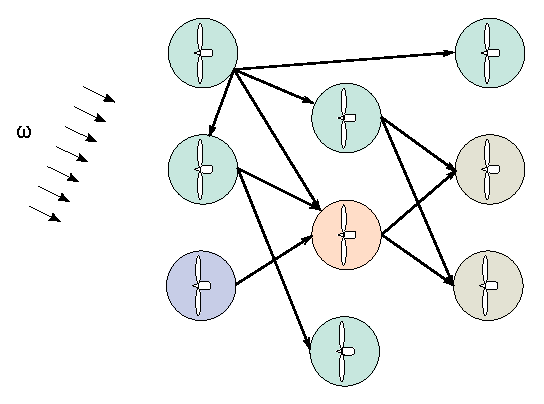
\includegraphics[width=0.4\columnwidth]{figs/graph/graph.eps}
\caption{A wind turbine (purple) and its descendants in a wind turbine interaction DAG}
\label{fig:graph}
\end{figure}

\clearpage

\section{Visual Overview of Layouts}\label{appendix:layouts}
\begin{figure}[!htb]
     \centering
     \begin{subfigure}{0.3\columnwidth}
      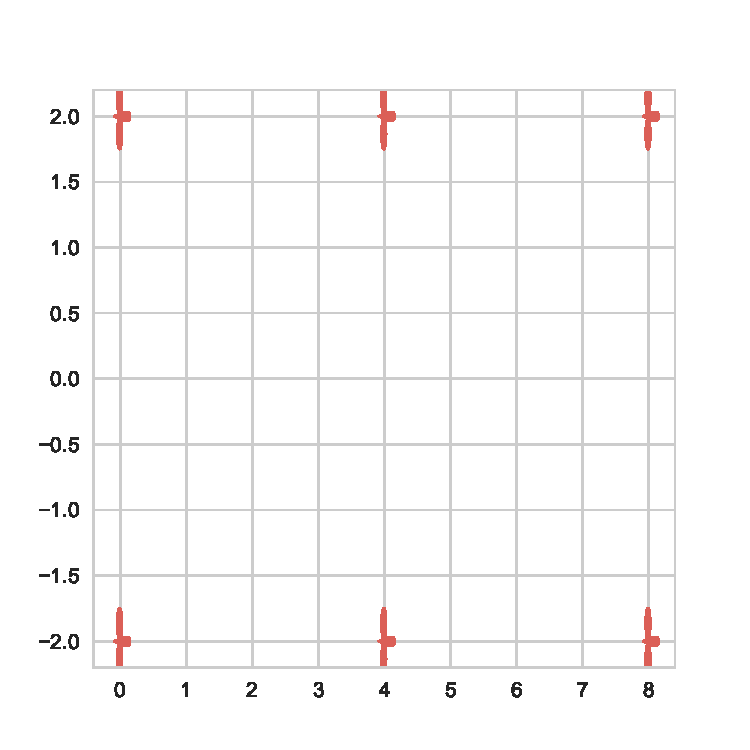
\includegraphics[width=\columnwidth]{figs/layouts/layoutTurb6_Row2.pdf}
     \caption{Turb6\_Row2: 6 turbines}
     \end{subfigure}
     \begin{subfigure}{0.3\columnwidth}
     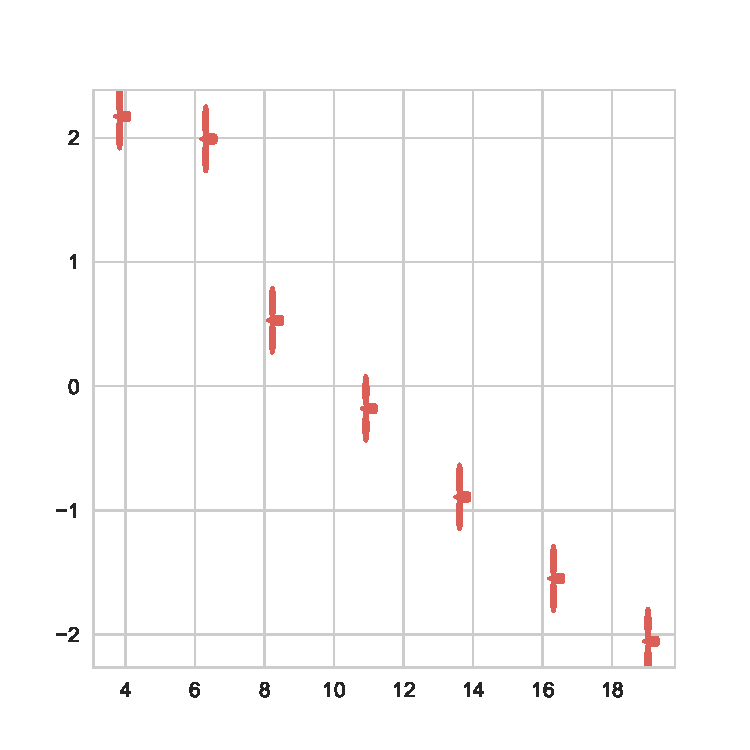
\includegraphics[width=\columnwidth]{figs/layouts/layoutAblaincourt.pdf}
     \caption{Ablaincourt: 7 turbines}
     \end{subfigure}
     \begin{subfigure}{0.3\columnwidth}
     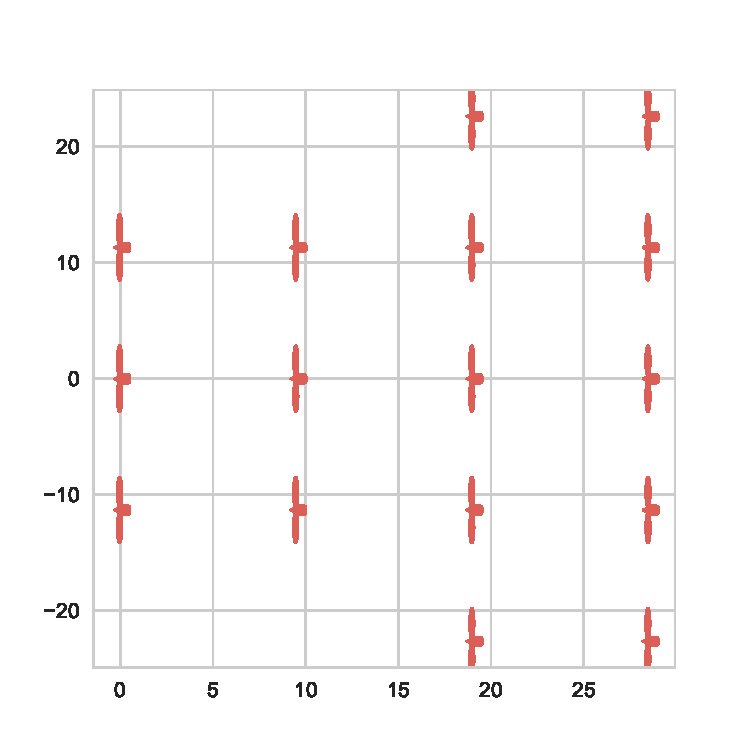
\includegraphics[width=\columnwidth]{figs/layouts/layoutTurb16_Row5.pdf}
     \caption{Turb16\_Row5: 16 turbines}
     \end{subfigure}
     \begin{subfigure}{0.3\columnwidth}
     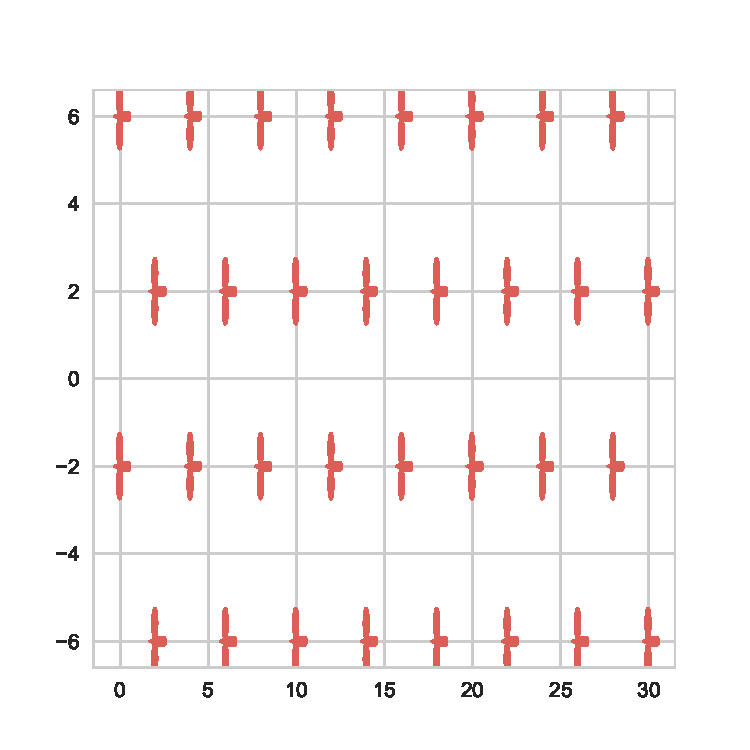
\includegraphics[width=\columnwidth]{figs/layouts/layoutTurb_TCRWP.pdf}
     \caption{Turb\_TCRWP: 32 turbines}
     \end{subfigure}
     \begin{subfigure}{0.3\columnwidth}
     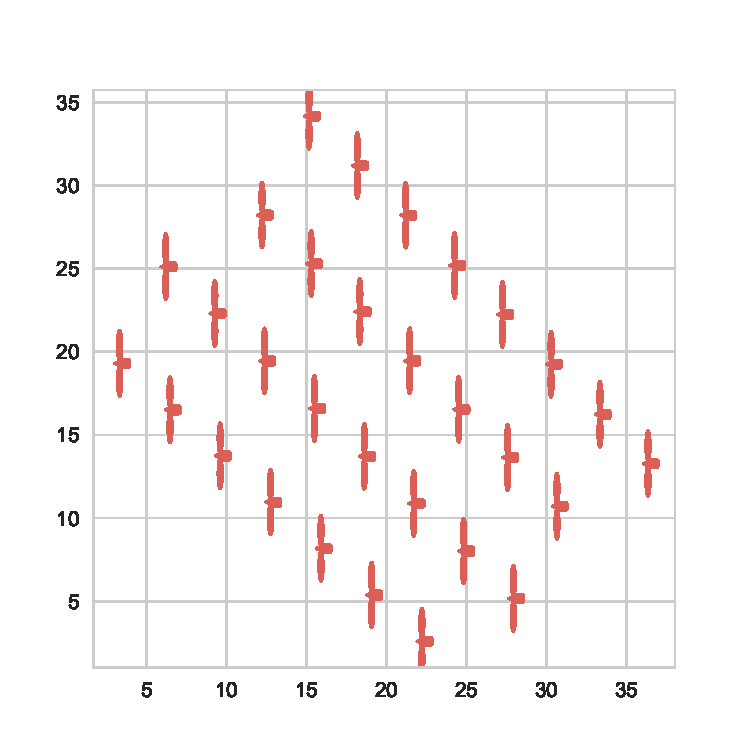
\includegraphics[width=\columnwidth]{figs/layouts/layoutOrmonde.pdf}
     \caption{Ormonde: 30 turbines}
     \end{subfigure}
    \begin{subfigure}{0.3\columnwidth}
     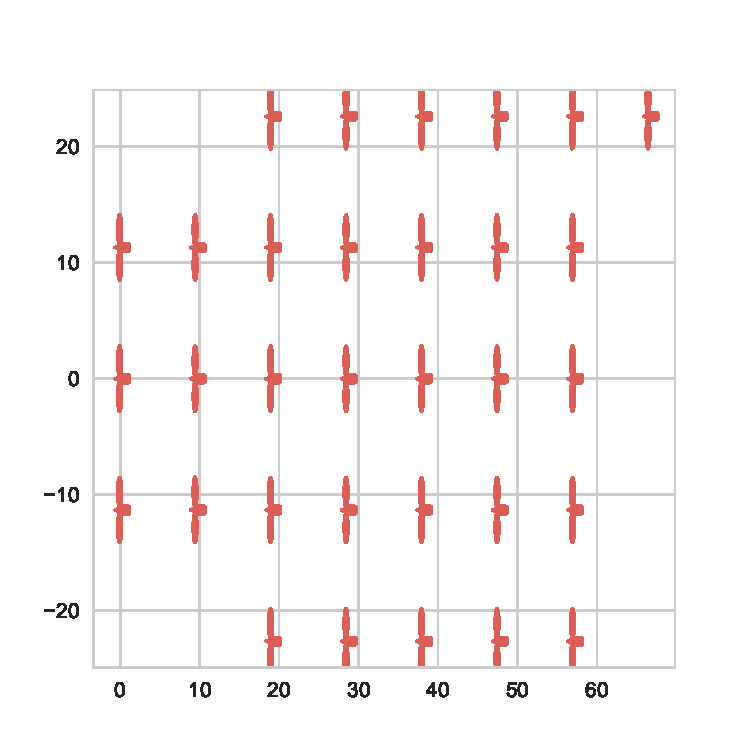
\includegraphics[width=\columnwidth]{figs/layouts/layoutTurb32_Row5.pdf}
     \caption{Turb32\_Row5: 32 turbines}
     \end{subfigure}
     \begin{subfigure}{0.3\columnwidth}
     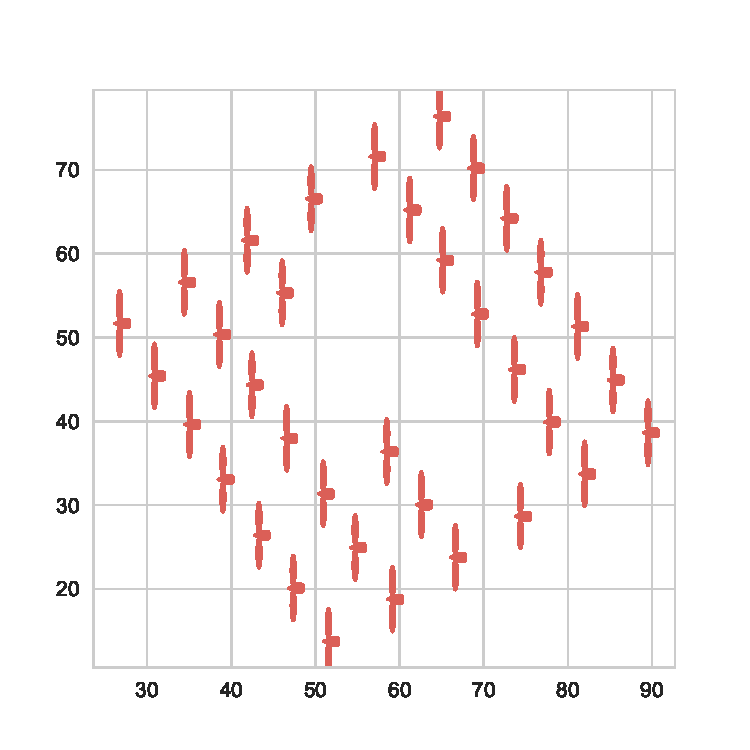
\includegraphics[width=\columnwidth]{figs/layouts/layoutWMR.pdf}
     \caption{WMR: 35 turbines}
     \end{subfigure}
    \begin{subfigure}{0.3\columnwidth}
     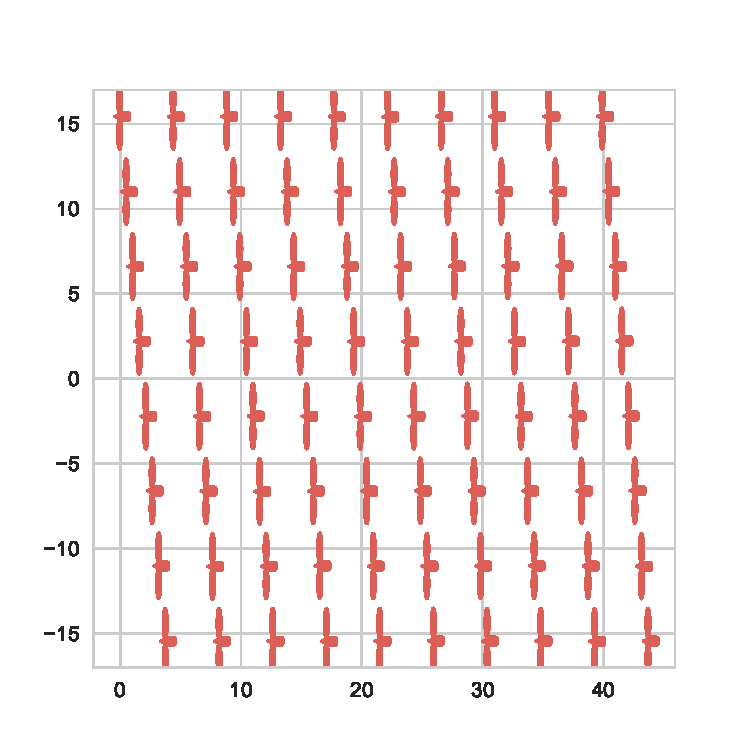
\includegraphics[width=\columnwidth]{figs/layouts/layoutHornsRev1.pdf}
     \caption{HornsRev1: 80 turbines}
     \end{subfigure}
    \begin{subfigure}{0.3\columnwidth}
     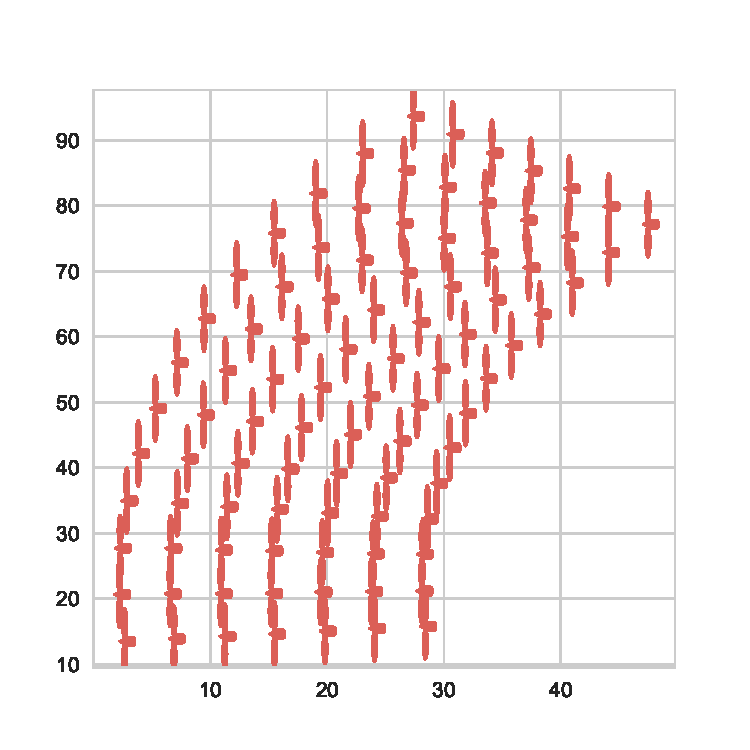
\includegraphics[width=\columnwidth]{figs/layouts/layoutHornsRev2.pdf}
     \caption{HornsRev2: 91 turbines}
     \end{subfigure}
     \begin{subfigure}{0.3\columnwidth}
     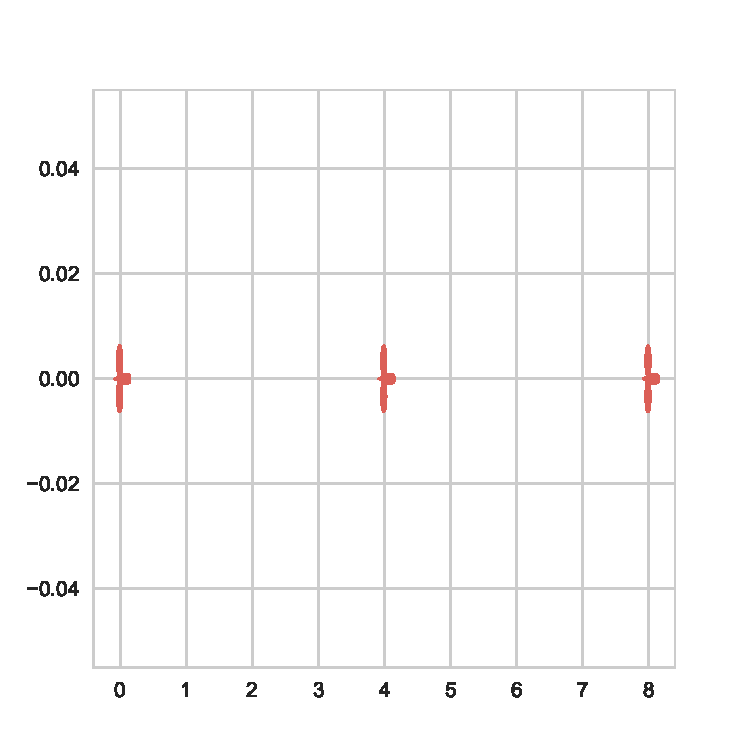
\includegraphics[width=\columnwidth]{figs/layouts/layoutTurb3_Row1.pdf}
     \caption{TurbX\_Row1. X = 3}
     \end{subfigure}
     \begin{subfigure}{0.3\columnwidth}
     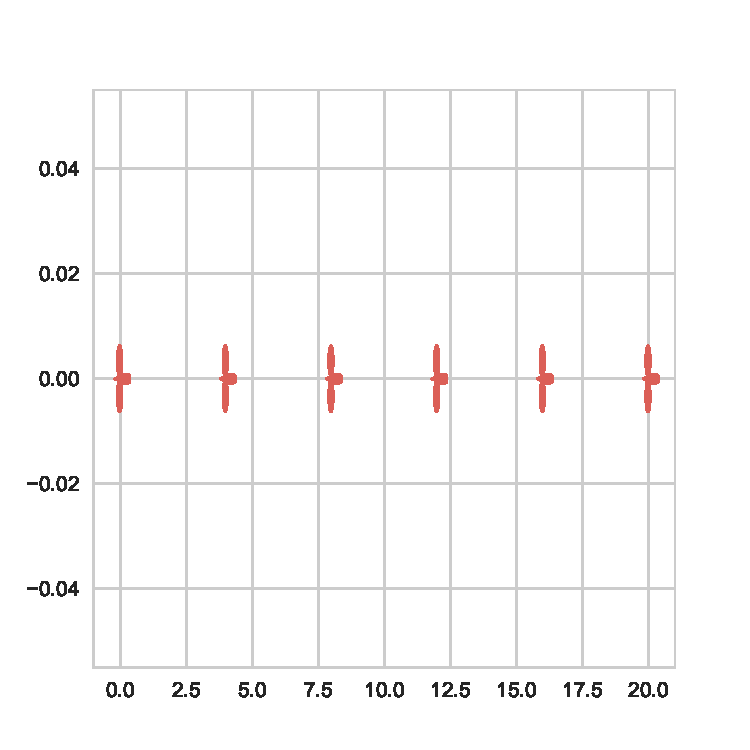
\includegraphics[width=\columnwidth]{figs/layouts/layoutTurb6_Row1.pdf}
     \caption{X=6}
     \end{subfigure}
     \begin{subfigure}{0.3\columnwidth}
     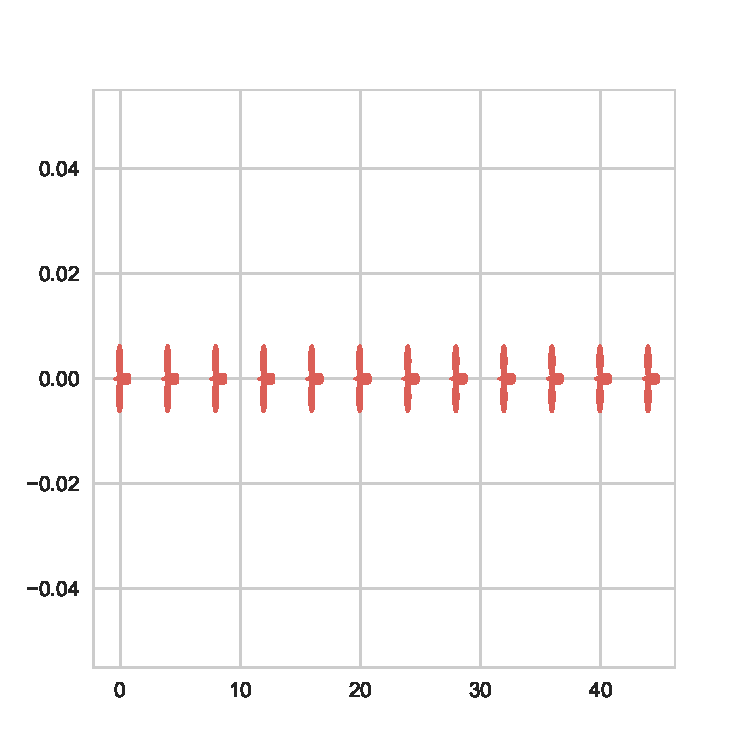
\includegraphics[width=\columnwidth]{figs/layouts/layoutTurb12_Row1.pdf}
     \caption{X = 12}
     \end{subfigure}
    % \begin{subfigure}{0.3\columnwidth}
    %  \includesvg[width=\columnwidth]{figs/layouts/layoutTurb1_Row1.svg}
    %  \caption{Turb1\_Row1: 1 turbines}
    %  \end{subfigure}
    % \begin{subfigure}{0.3\columnwidth}
    %  \includesvg[width=\columnwidth]{figs/layouts/layoutTurb2_Row1.svg}
    %  \caption{Turb2\_Row1: 2 turbines}
    %  \end{subfigure}
    % \begin{subfigure}{0.3\columnwidth}
    %  \includesvg[width=\columnwidth]{figs/layouts/layoutTurb3_Row1.svg}
    %  \caption{Turb3\_Row1: 3 turbines}
    %  \end{subfigure}
    % \begin{subfigure}{0.3\columnwidth}
    %  \includesvg[width=\columnwidth]{figs/layouts/layoutTurb4_Row1.svg}
    %  \caption{Turb4\_Row1: 4 turbines}
    %  \end{subfigure}
    % \begin{subfigure}{0.3\columnwidth}
    %  \includesvg[width=\columnwidth]{figs/layouts/layoutTurb5_Row1.svg}
    %  \caption{Turb5\_Row1: 5 turbines}
    %  \end{subfigure}
    % \begin{subfigure}{0.3\columnwidth}
    %  \includesvg[width=\columnwidth]{figs/layouts/layoutTurb6_Row1.svg}
    %  \caption{Turb6\_Row1: 6 turbines}
    %  \end{subfigure}
    % \begin{subfigure}{0.3\columnwidth}
    %  \includesvg[width=\columnwidth]{figs/layouts/layoutTurb7_Row1.svg}
    %  \caption{Turb7\_Row1: 7 turbines}
    %  \end{subfigure}
    % \begin{subfigure}{0.3\columnwidth}
    %  \includesvg[width=\columnwidth]{figs/layouts/layoutTurb8_Row1.svg}
    %  \caption{Turb8\_Row1: 8 turbines}
    %  \end{subfigure}
    % \begin{subfigure}{0.3\columnwidth}
    %  \includesvg[width=\columnwidth]{figs/layouts/layoutTurb9_Row1.svg}
    %  \caption{Turb9\_Row1: 9 turbines}
    %  \end{subfigure}
    % \begin{subfigure}{0.3\columnwidth}
    %  \includesvg[width=\columnwidth]{figs/layouts/layoutTurb10_Row1.svg}
    %  \caption{Turb10\_Row1: 10 turbines}
    %  \end{subfigure}
    % \begin{subfigure}{0.3\columnwidth}
    %  \includesvg[width=\columnwidth]{figs/layouts/layoutTurb11_Row1.svg}
    %  \caption{Turb11\_Row1: 11 turbines}
    %  \end{subfigure}
    % \begin{subfigure}{0.3\columnwidth}
    %  \includesvg[width=\columnwidth]{figs/layouts/layoutTurb12_Row1.svg}
    %  \caption{Turb12\_Row1: 12 turbines}
    %  \end{subfigure}
     % \begin{subfigure}{0.3\columnwidth}
     % \includesvg[width=\columnwidth]{figs/layouts/layout3TurbRow1.svg}
     % \caption{Toy case: Row of $3$ turbines}
     % \end{subfigure}
     % \begin{subfigure}{0.3\columnwidth}
     % \includesvg[width=\columnwidth]{figs/layouts/layoutAblaincourt.svg}
     % \caption{Ablaincourt}
     % \end{subfigure}
     % \begin{subfigure}{0.3\columnwidth}
     % \includesvg[width=\columnwidth]{figs/layouts/layoutOrmonde.svg}
     % \caption{Ormonde}
     % \end{subfigure}
     % \begin{subfigure}{0.3\columnwidth}
     % \includesvg[width=\columnwidth]{figs/layouts/layoutWMR.svg}
     % \caption{WMR}
     % \end{subfigure}
     %  \begin{subfigure}{0.3\columnwidth}
     % \includesvg[width=\columnwidth]{figs/layouts/layoutHornsRev1.svg}
     % \caption{Horns Rev 1}
     % \end{subfigure}
     % \begin{subfigure}{0.3\columnwidth}
     % \includesvg[width=\columnwidth]{figs/layouts/layoutHornsRev2.svg}
     % \caption{Horns Rev 2}
     % \end{subfigure}
\caption{Coordinates of each wind turbine for the pre-registered layouts in WFCRL. %Distances are in $km$ and the distance between two adjacent grid lines (resp. columns) is of $1$ turbine diameter.
Distances are in turbine diameters ($126m$ for the NREL 5MW Reference turbine). The \textit{TurbX\_Row1} toy layouts are procedurally generated for any value of $X$ between $1$ and $12$.}
 \label{fig:layouts}
\end{figure}

\newpage


\section{Additional information on WFCRL}
\subsection{List of dependencies}\label{appendix:dependencies}

We report in the table below the list of open-source Python packages and other open-source software that WCFRL relies on.

% Please add the following required packages to your document preamble:
% \usepackage[normalem]{ulem}
% \useunder{\uline}{\ul}{}
% Please add the following required packages to your document preamble:
% \usepackage[normalem]{ulem}
% \useunder{\uline}{\ul}{}
\begin{table}[!htb]
\resizebox{1.15\columnwidth}{!}{%
\begin{tabular}{lcl}
\textbf{Software}    & \multicolumn{1}{l}{\textbf{License}} & \textbf{License Link}                                                  \\
numpy                & \textit{Custom}                      & \url{https://numpy.org/doc/stable/license.html}                           \\
Gymnasium            & MIT                          & \url{https://github.com/Farama-Foundation/Gymnasium/blob/main/LICENSE}    \\
PettingZoo           & MIT                          & \url{https://github.com/Farama-Foundation/PettingZoo/blob/master/LICENSE} \\
FLORIS               & Apache v2.0                          & \url{https://github.com/NREL/floris/blob/main/LICENSE.txt}                \\
FAST.Farm (OpenFAST) & Apache v2.0                          & \url{https://github.com/OpenFAST/openfast/blob/main/LICENSE}              \\
mpi4py               & \textit{Custom}                      & \url{https://github.com/erdc/mpi4py/blob/master/LICENSE.txt}              \\
Microsoft-MPI        & MIT                          & \url{https://github.com/microsoft/Microsoft-MPI/blob/master/LICENSE.txt}  \\
Open MPI             & BSD 3-Clause                         & \url{https://www.open-mpi.org/community/license.php}    \\
Seaborn             & BSD 3-Clause                         & \url{https://github.com/mwaskom/seaborn/blob/master/LICENSE.md} \\
Matplotlib & \textit{Custom} - BSD-compatible &
\url{https://matplotlib.org/stable/project/license.html} \\
PyYAML & MIT &
\url{https://github.com/yaml/pyyaml/blob/main/LICENSE} \\
Pandas             & BSD 3-Clause                         & \url{https://github.com/pandas-dev/pandas/blob/main/LICENSE} \\
\end{tabular}}
\label{tab:dependencies}
\end{table}

\subsection{Licence}\label{appendix:licence}

The WFCRL package is licensed under the Apache v2 license. The text of the license can be found here: \url{https://github.com/ifpen/wfcrl-env/blob/main/LICENSE}.
%We report it below:

% \begin{displayquote}

%                                 Apache License
%                         Version 2.0, January 2004
%                     http://www.apache.org/licenses/

% TERMS AND CONDITIONS FOR USE, REPRODUCTION, AND DISTRIBUTION

% 1. Definitions.

%     "License" shall mean the terms and conditions for use, reproduction,
%     and distribution as defined by Sections 1 through 9 of this document.

%     "Licensor" shall mean the copyright owner or entity authorized by
%     the copyright owner that is granting the License.

%     "Legal Entity" shall mean the union of the acting entity and all
%     other entities that control, are controlled by, or are under common
%     control with that entity. For the purposes of this definition,
%     "control" means (i) the power, direct or indirect, to cause the
%     direction or management of such entity, whether by contract or
%     otherwise, or (ii) ownership of fifty percent (50%) or more of the
%     outstanding shares, or (iii) beneficial ownership of such entity.

%     "You" (or "Your") shall mean an individual or Legal Entity
%     exercising permissions granted by this License.

%     "Source" form shall mean the preferred form for making modifications,
%     including but not limited to software source code, documentation
%     source, and configuration files.

%     "Object" form shall mean any form resulting from mechanical
%     transformation or translation of a Source form, including but
%     not limited to compiled object code, generated documentation,
%     and conversions to other media types.

%     "Work" shall mean the work of authorship, whether in Source or
%     Object form, made available under the License, as indicated by a
%     copyright notice that is included in or attached to the work
%     (an example is provided in the Appendix below).

%     "Derivative Works" shall mean any work, whether in Source or Object
%     form, that is based on (or derived from) the Work and for which the
%     editorial revisions, annotations, elaborations, or other modifications
%     represent, as a whole, an original work of authorship. For the purposes
%     of this License, Derivative Works shall not include works that remain
%     separable from, or merely link (or bind by name) to the interfaces of,
%     the Work and Derivative Works thereof.

%     "Contribution" shall mean any work of authorship, including
%     the original version of the Work and any modifications or additions
%     to that Work or Derivative Works thereof, that is intentionally
%     submitted to Licensor for inclusion in the Work by the copyright owner
%     or by an individual or Legal Entity authorized to submit on behalf of
%     the copyright owner. For the purposes of this definition, "submitted"
%     means any form of electronic, verbal, or written communication sent
%     to the Licensor or its representatives, including but not limited to
%     communication on electronic mailing lists, source code control systems,
%     and issue tracking systems that are managed by, or on behalf of, the
%     Licensor for the purpose of discussing and improving the Work, but
%     excluding communication that is conspicuously marked or otherwise
%     designated in writing by the copyright owner as "Not a Contribution."

%     "Contributor" shall mean Licensor and any individual or Legal Entity
%     on behalf of whom a Contribution has been received by Licensor and
%     subsequently incorporated within the Work.

% 2. Grant of Copyright License. Subject to the terms and conditions of
%     this License, each Contributor hereby grants to You a perpetual,
%     worldwide, non-exclusive, no-charge, royalty-free, irrevocable
%     copyright license to reproduce, prepare Derivative Works of,
%     publicly display, publicly perform, sublicense, and distribute the
%     Work and such Derivative Works in Source or Object form.

% 3. Grant of Patent License. Subject to the terms and conditions of
%     this License, each Contributor hereby grants to You a perpetual,
%     worldwide, non-exclusive, no-charge, royalty-free, irrevocable
%     (except as stated in this section) patent license to make, have made,
%     use, offer to sell, sell, import, and otherwise transfer the Work,
%     where such license applies only to those patent claims licensable
%     by such Contributor that are necessarily infringed by their
%     Contribution(s) alone or by combination of their Contribution(s)
%     with the Work to which such Contribution(s) was submitted. If You
%     institute patent litigation against any entity (including a
%     cross-claim or counterclaim in a lawsuit) alleging that the Work
%     or a Contribution incorporated within the Work constitutes direct
%     or contributory patent infringement, then any patent licenses
%     granted to You under this License for that Work shall terminate
%     as of the date such litigation is filed.

% 4. Redistribution. You may reproduce and distribute copies of the
%     Work or Derivative Works thereof in any medium, with or without
%     modifications, and in Source or Object form, provided that You
%     meet the following conditions:

%     (a) You must give any other recipients of the Work or
%         Derivative Works a copy of this License; and

%     (b) You must cause any modified files to carry prominent notices
%         stating that You changed the files; and

%     (c) You must retain, in the Source form of any Derivative Works
%         that You distribute, all copyright, patent, trademark, and
%         attribution notices from the Source form of the Work,
%         excluding those notices that do not pertain to any part of
%         the Derivative Works; and

%     (d) If the Work includes a "NOTICE" text file as part of its
%         distribution, then any Derivative Works that You distribute must
%         include a readable copy of the attribution notices contained
%         within such NOTICE file, excluding those notices that do not
%         pertain to any part of the Derivative Works, in at least one
%         of the following places: within a NOTICE text file distributed
%         as part of the Derivative Works; within the Source form or
%         documentation, if provided along with the Derivative Works; or,
%         within a display generated by the Derivative Works, if and
%         wherever such third-party notices normally appear. The contents
%         of the NOTICE file are for informational purposes only and
%         do not modify the License. You may add Your own attribution
%         notices within Derivative Works that You distribute, alongside
%         or as an addendum to the NOTICE text from the Work, provided
%         that such additional attribution notices cannot be construed
%         as modifying the License.

%     You may add Your own copyright statement to Your modifications and
%     may provide additional or different license terms and conditions
%     for use, reproduction, or distribution of Your modifications, or
%     for any such Derivative Works as a whole, provided Your use,
%     reproduction, and distribution of the Work otherwise complies with
%     the conditions stated in this License.

% 5. Submission of Contributions. Unless You explicitly state otherwise,
%     any Contribution intentionally submitted for inclusion in the Work
%     by You to the Licensor shall be under the terms and conditions of
%     this License, without any additional terms or conditions.
%     Notwithstanding the above, nothing herein shall supersede or modify
%     the terms of any separate license agreement you may have executed
%     with Licensor regarding such Contributions.

% 6. Trademarks. This License does not grant permission to use the trade
%     names, trademarks, service marks, or product names of the Licensor,
%     except as required for reasonable and customary use in describing the
%     origin of the Work and reproducing the content of the NOTICE file.

% 7. Disclaimer of Warranty. Unless required by applicable law or
%     agreed to in writing, Licensor provides the Work (and each
%     Contributor provides its Contributions) on an "AS IS" BASIS,
%     WITHOUT WARRANTIES OR CONDITIONS OF ANY KIND, either express or
%     implied, including, without limitation, any warranties or conditions
%     of TITLE, NON-INFRINGEMENT, MERCHANTABILITY, or FITNESS FOR A
%     PARTICULAR PURPOSE. You are solely responsible for determining the
%     appropriateness of using or redistributing the Work and assume any
%     risks associated with Your exercise of permissions under this License.

% 8. Limitation of Liability. In no event and under no legal theory,
%     whether in tort (including negligence), contract, or otherwise,
%     unless required by applicable law (such as deliberate and grossly
%     negligent acts) or agreed to in writing, shall any Contributor be
%     liable to You for damages, including any direct, indirect, special,
%     incidental, or consequential damages of any character arising as a
%     result of this License or out of the use or inability to use the
%     Work (including but not limited to damages for loss of goodwill,
%     work stoppage, computer failure or malfunction, or any and all
%     other commercial damages or losses), even if such Contributor
%     has been advised of the possibility of such damages.

% 9. Accepting Warranty or Additional Liability. While redistributing
%     the Work or Derivative Works thereof, You may choose to offer,
%     and charge a fee for, acceptance of support, warranty, indemnity,
%     or other liability obligations and/or rights consistent with this
%     License. However, in accepting such obligations, You may act only
%     on Your own behalf and on Your sole responsibility, not on behalf
%     of any other Contributor, and only if You agree to indemnify,
%     defend, and hold each Contributor harmless for any liability
%     incurred by, or claims asserted against, such Contributor by reason
%     of your accepting any such warranty or additional liability.

% END OF TERMS AND CONDITIONS
% \end{displayquote}

\subsection{Responsability}
The authors bear all responsibility in case of violation of rights.

\end{document}
